\documentclass{ase}

\usepackage{graphicx}
\usepackage{acronym}
\usepackage{cleveref}
\usepackage{listings}
\usepackage{hyperref}
\usepackage{vdmlisting}
\usepackage{appendix}
\usepackage{xspace}
\usepackage{amsmath}
\usepackage{textcomp}
\usepackage[framemethod=TikZ]{mdframed}
\usepackage{fixltx2e} % For subscript command
\usepackage{todonotes}
\presetkeys{todonotes}{inline,linecolor=red,backgroundcolor=blue!20!white, bordercolor=red}{}

% To get cref to work with appendices
\crefname{app}{appendix}{appendices}
\Crefname{app}{Appendix}{Appendices}

% Including times to make bold facing of keywords work for ttfamily in JML listings
% \usepackage{times}
% @(#)$Id: jml-listings.tex,v 1.7 2010/02/25 21:57:06 leavens Exp $
%
% Copyright (C) 2006 Iowa State University
%
% This file is part of JML
%
% JML is free software; you can redistribute it and/or modify
% it under the terms of the GNU General Public License as published by
% the Free Software Foundation; either version 2, or (at your option)
% any later version.
%
% JML is distributed in the hope that it will be useful,
% but WITHOUT ANY WARRANTY; without even the implied warranty of
% MERCHANTABILITY or FITNESS FOR A PARTICULAR PURPOSE.  See the
% GNU General Public License for more details.
%
% You should have received a copy of the GNU General Public License
% along with JML; see the file COPYING.  If not, write to
% the Free Software Foundation, 675 Mass Ave, Cambridge, MA 02139, USA.
%
% A JML listings environment.
%
% AUTHOR: Gary T. Leavens
%
% requires listings i.e., do \usepackage{listings} first
%
% This file is set up to be used via % @(#)$Id: jml-listings.tex,v 1.7 2010/02/25 21:57:06 leavens Exp $
%
% Copyright (C) 2006 Iowa State University
%
% This file is part of JML
%
% JML is free software; you can redistribute it and/or modify
% it under the terms of the GNU General Public License as published by
% the Free Software Foundation; either version 2, or (at your option)
% any later version.
%
% JML is distributed in the hope that it will be useful,
% but WITHOUT ANY WARRANTY; without even the implied warranty of
% MERCHANTABILITY or FITNESS FOR A PARTICULAR PURPOSE.  See the
% GNU General Public License for more details.
%
% You should have received a copy of the GNU General Public License
% along with JML; see the file COPYING.  If not, write to
% the Free Software Foundation, 675 Mass Ave, Cambridge, MA 02139, USA.
%
% A JML listings environment.
%
% AUTHOR: Gary T. Leavens
%
% requires listings i.e., do \usepackage{listings} first
%
% This file is set up to be used via % @(#)$Id: jml-listings.tex,v 1.7 2010/02/25 21:57:06 leavens Exp $
%
% Copyright (C) 2006 Iowa State University
%
% This file is part of JML
%
% JML is free software; you can redistribute it and/or modify
% it under the terms of the GNU General Public License as published by
% the Free Software Foundation; either version 2, or (at your option)
% any later version.
%
% JML is distributed in the hope that it will be useful,
% but WITHOUT ANY WARRANTY; without even the implied warranty of
% MERCHANTABILITY or FITNESS FOR A PARTICULAR PURPOSE.  See the
% GNU General Public License for more details.
%
% You should have received a copy of the GNU General Public License
% along with JML; see the file COPYING.  If not, write to
% the Free Software Foundation, 675 Mass Ave, Cambridge, MA 02139, USA.
%
% A JML listings environment.
%
% AUTHOR: Gary T. Leavens
%
% requires listings i.e., do \usepackage{listings} first
%
% This file is set up to be used via \input{jml-listings}.
% Typically one would use \lstset{language=[JML]Java}
% to make the JML dialect of the Java language active, although there
% are other ways to do that in the listings package.
% If you want, you could make a version that is a style file,
% but then change \lstdefinelanguage to \lst@definelanguage below.
%
\lstdefinelanguage[JML]{Java}[]{Java}%
       {% C++ style comments have to start with a blank!
        comment=[l]{//\ },
        % And C-style comments must also start with a blank or star!
        morecomment=[s]{/*\ }{*/},        
        morecomment=[s]{/**}{*/},
        % sensitive=true, % inherited
        % Add JML keywords as level 1 keywords, so can typeset differently
        classoffset=1,
        % And here are all the wonderful JML keywords
        morekeywords={abrupt_behavior,abrupt_behaviour,
         accessible,accessible_redundantly,also,assert,assert_redundantly,
         assignable,assignable_redundantly,assume,assume_redundantly,
         axiom,behavior,behaviour,breaks,breaks_redundantly,
         callable,callable_redundantly,captures,captures_redundantly,
         choose,choose_if,code,code_bigint_math,code_java_math,
         code_safe_math,constraint,constraint_redundantly,constructor,
         continues,continues_redundantly,decreases,decreases_redundantly,
         decreasing,decreasing_redundantly,diverges,diverges_redundantly,
         duration,duration_redundantly,ensures,ensures_redundantly,
         example,exceptional_behavior,exceptional_behaviour,
         exceptional_example,exsures,exsures_redundantly,extract,field,
         forall,for_example,ghost,helper,hence_by,hence_by_redundantly,
         implies_that,in,in_redundantly,initializer,initially,instance,
         invariant,invariant_redundantly,loop_invariant,
         loop_invariant_redundantly,maintaining,maintaining_redundantly,
         maps,maps_redundantly,measured_by,measured_by_redundantly,method,
         model,model_program,modifiable,modifiable_redundantly,modifies,
         modifies_redundantly,monitored,monitors_for,non_null,
         normal_behavior,normal_behaviour,normal_example,nowarn,
         nullable,nullable_by_default,old,or,post,post_redundantly,
         pre,pre_redundantly,pure,readable,refine,refines,refining,represents,
         represents_redundantly,requires,requires_redundantly,
         returns,returns_redundantly,set,signals,signals_only,
         signals_only_redundantly,signals_redundantly,spec_bigint_math,
         spec_java_math,spec_protected,spec_public,spec_safe_math,
         static_initializer,uninitialized,unreachable,weakly,
         when,when_redundantly,working_space,working_space_redundantly,
         writable
        },
        % keywords from the universe type system
        morekeywords={rep,peer,readonly},
        % typeset everything that starts with a backslash as a keyword
        % BUG: this doesn't allow typesetting these keywords differently
        keywordsprefix=\\,
        otherkeywords={<:,<-,->,..,<==,==>,<==>,<=!=>},
        classoffset=0 % restore default class for keywords
}
.
% Typically one would use \lstset{language=[JML]Java}
% to make the JML dialect of the Java language active, although there
% are other ways to do that in the listings package.
% If you want, you could make a version that is a style file,
% but then change \lstdefinelanguage to \lst@definelanguage below.
%
\lstdefinelanguage[JML]{Java}[]{Java}%
       {% C++ style comments have to start with a blank!
        comment=[l]{//\ },
        % And C-style comments must also start with a blank or star!
        morecomment=[s]{/*\ }{*/},        
        morecomment=[s]{/**}{*/},
        % sensitive=true, % inherited
        % Add JML keywords as level 1 keywords, so can typeset differently
        classoffset=1,
        % And here are all the wonderful JML keywords
        morekeywords={abrupt_behavior,abrupt_behaviour,
         accessible,accessible_redundantly,also,assert,assert_redundantly,
         assignable,assignable_redundantly,assume,assume_redundantly,
         axiom,behavior,behaviour,breaks,breaks_redundantly,
         callable,callable_redundantly,captures,captures_redundantly,
         choose,choose_if,code,code_bigint_math,code_java_math,
         code_safe_math,constraint,constraint_redundantly,constructor,
         continues,continues_redundantly,decreases,decreases_redundantly,
         decreasing,decreasing_redundantly,diverges,diverges_redundantly,
         duration,duration_redundantly,ensures,ensures_redundantly,
         example,exceptional_behavior,exceptional_behaviour,
         exceptional_example,exsures,exsures_redundantly,extract,field,
         forall,for_example,ghost,helper,hence_by,hence_by_redundantly,
         implies_that,in,in_redundantly,initializer,initially,instance,
         invariant,invariant_redundantly,loop_invariant,
         loop_invariant_redundantly,maintaining,maintaining_redundantly,
         maps,maps_redundantly,measured_by,measured_by_redundantly,method,
         model,model_program,modifiable,modifiable_redundantly,modifies,
         modifies_redundantly,monitored,monitors_for,non_null,
         normal_behavior,normal_behaviour,normal_example,nowarn,
         nullable,nullable_by_default,old,or,post,post_redundantly,
         pre,pre_redundantly,pure,readable,refine,refines,refining,represents,
         represents_redundantly,requires,requires_redundantly,
         returns,returns_redundantly,set,signals,signals_only,
         signals_only_redundantly,signals_redundantly,spec_bigint_math,
         spec_java_math,spec_protected,spec_public,spec_safe_math,
         static_initializer,uninitialized,unreachable,weakly,
         when,when_redundantly,working_space,working_space_redundantly,
         writable
        },
        % keywords from the universe type system
        morekeywords={rep,peer,readonly},
        % typeset everything that starts with a backslash as a keyword
        % BUG: this doesn't allow typesetting these keywords differently
        keywordsprefix=\\,
        otherkeywords={<:,<-,->,..,<==,==>,<==>,<=!=>},
        classoffset=0 % restore default class for keywords
}
.
% Typically one would use \lstset{language=[JML]Java}
% to make the JML dialect of the Java language active, although there
% are other ways to do that in the listings package.
% If you want, you could make a version that is a style file,
% but then change \lstdefinelanguage to \lst@definelanguage below.
%
\lstdefinelanguage[JML]{Java}[]{Java}%
       {% C++ style comments have to start with a blank!
        comment=[l]{//\ },
        % And C-style comments must also start with a blank or star!
        morecomment=[s]{/*\ }{*/},        
        morecomment=[s]{/**}{*/},
        % sensitive=true, % inherited
        % Add JML keywords as level 1 keywords, so can typeset differently
        classoffset=1,
        % And here are all the wonderful JML keywords
        morekeywords={abrupt_behavior,abrupt_behaviour,
         accessible,accessible_redundantly,also,assert,assert_redundantly,
         assignable,assignable_redundantly,assume,assume_redundantly,
         axiom,behavior,behaviour,breaks,breaks_redundantly,
         callable,callable_redundantly,captures,captures_redundantly,
         choose,choose_if,code,code_bigint_math,code_java_math,
         code_safe_math,constraint,constraint_redundantly,constructor,
         continues,continues_redundantly,decreases,decreases_redundantly,
         decreasing,decreasing_redundantly,diverges,diverges_redundantly,
         duration,duration_redundantly,ensures,ensures_redundantly,
         example,exceptional_behavior,exceptional_behaviour,
         exceptional_example,exsures,exsures_redundantly,extract,field,
         forall,for_example,ghost,helper,hence_by,hence_by_redundantly,
         implies_that,in,in_redundantly,initializer,initially,instance,
         invariant,invariant_redundantly,loop_invariant,
         loop_invariant_redundantly,maintaining,maintaining_redundantly,
         maps,maps_redundantly,measured_by,measured_by_redundantly,method,
         model,model_program,modifiable,modifiable_redundantly,modifies,
         modifies_redundantly,monitored,monitors_for,non_null,
         normal_behavior,normal_behaviour,normal_example,nowarn,
         nullable,nullable_by_default,old,or,post,post_redundantly,
         pre,pre_redundantly,pure,readable,refine,refines,refining,represents,
         represents_redundantly,requires,requires_redundantly,
         returns,returns_redundantly,set,signals,signals_only,
         signals_only_redundantly,signals_redundantly,spec_bigint_math,
         spec_java_math,spec_protected,spec_public,spec_safe_math,
         static_initializer,uninitialized,unreachable,weakly,
         when,when_redundantly,working_space,working_space_redundantly,
         writable
        },
        % keywords from the universe type system
        morekeywords={rep,peer,readonly},
        % typeset everything that starts with a backslash as a keyword
        % BUG: this doesn't allow typesetting these keywords differently
        keywordsprefix=\\,
        otherkeywords={<:,<-,->,..,<==,==>,<==>,<=!=>},
        classoffset=0 % restore default class for keywords
}


\acrodef{ast}[AST]{Abstract Syntax Tree}
\acrodef{fad}[FAD]{Financial Accounting District}
\acrodef{vdm}[VDM]{the Vienna Development Method}
\acrodef{vdmsl}[VDM-SL]{the Vienna Development Method Specification Language}
\acrodef{jml}[JML]{the Java Modeling Language}
\acrodef{dbc}[DbC]{Design-by-Contract}
\acrodef{atm}[ATM]{Automated Teller Machine}
\acrodef{pvs}[PVS]{the Prototype Verification System}
\acrodef{uml}[UML]{the Unified Modeling Language}
\acrodef{ir}[IR]{Intermediate Representation}

\newcommand{\vsl}{VDM-SL\xspace}

\lstset
{
  basicstyle=\footnotesize\ttfamily,
  numbers=left,
  firstnumber=1,
  numberfirstline=true,
  xleftmargin=1.5em
}

% Used by the VDM listings in the appendices
\lstdefinestyle{appendixVdm}
{
  frame=trBL,
  frameround=fttt  
}

% Custom VDM style (used by the listings in chapters/sections)
\lstdefinestyle{customVdm}
{
  escapechar=!,
  breaklines=true,
  basicstyle=\footnotesize\ttfamily,
  % frame=single,
  % frameround=,
  linewidth=\columnwidth,
  morekeywords={atomic},
  moredelim={[is][keywordstyle]{@}{@}}
}


% Custom JML style
\lstdefinestyle{customJml}
{
  escapechar=~,
  breaklines=true,
  basicstyle=\footnotesize\ttfamily,
  language=[JML]Java,
  frame=tlrb,
  captionpos=b
}

% OpenJML RAC output
\lstdefinestyle{racOutput}
{
  %escapechar=!,
  captionpos=b,
  xleftmargin=0em,
  frame=single,
  numbers=none,
  breaklines=true,
  basicstyle=\footnotesize\ttfamily
}

\mdfdefinestyle{MyFrame}{%
    linecolor=black,
    outerlinewidth=1pt,
    frametitlerule=true,
    frametitlerulewidth=1pt,
    linewidth=0pt,
    roundcorner=0pt,
    innertopmargin=3pt,
    innerbottommargin=3pt,
    innerrightmargin=3pt,
    innerleftmargin=3pt,
    backgroundcolor=gray!20!white}

\newcounter{transRule}
\setcounter{transRule}{0}

\newcommand{\transRule}[2]{ \refstepcounter{transRule}%
  \begin{mdframed}[nobreak=true,style=MyFrame,frametitle=\arabic{transRule}. #1]
    #2
  \end{mdframed}}


\newcommand{\sub}[1]{\textsubscript{#1}}

\newcommand{\kw}[1]{\texttt{\textbf{#1}}\xspace}

% Definitions related to JML
\newcommand{\old}{\textbackslash \kw{old}}
\newcommand{\past}{\textbackslash \kw{past}}
\newcommand{\RESULT}{\textbackslash \kw{result}}
\newcommand{\JMLforall}{\textbackslash \kw{forall}}
\newcommand{\JMLexists}{\textbackslash \kw{exists}}

\newcommand{\invariantfor}{\textbackslash \kw{invariant\_for}}

\newcommand{\oldexp}[1]{\old(\texttt{#1})}

\newcommand{\inv}[1]{\texttt{\textbackslash \textbf{invariant\_for}(#1)}}

% Increase size of sub scripts
\DeclareMathSizes{10}{10}{9}{10}

% Example: d instance of D ==> \invariant for((D) d)
\newcommand{\guardedinv}[2]{\texttt{#1 \kw{instance} \kw{of} #2 ==>\\ \indent \textbackslash \textbf{invariant\_for}((#2) #1)}}

\title{Automated translation of VDM-SL to JML-annotated Java}
\subtitle{Technical Report}

\author{Peter W. V. Tran-J\o{}rgensen\\Peter Gorm
  Larsen\\GaryT. Leavens}

\reportid{TR-XX}
\frontlogo{figs/logo}
%\makenomenclature
\begin{document}

\maketitle
\frontmatter
\asetableofcontents

\mainmatter


\chapter{Introduction}

A model specified using the \ac{vdm} can be validated against its
contract-based elements (e.g.\ pre and postconditions and invariants)
in order to ensure that the system behaves as intended. One way to
validate the model against its contracts is by animation using
Overture's \ac{vdm} interpreter.

When sufficient insight into the system under development has been
obtained during the formal analysis, development proceeds to the
implementation phase, where the system is realised. One way to realise
a \ac{vdm} model is by implementing it in a programming language, for
example, using code generation. However, since no guarantees are made
about the correctness of the generated code, other measures must be
taken to increase the confidence in the correctness of the generated
code.

To support this approach, Overture enables fully automated translation
of \vsl's contract-based elements (pre- and postconditions, and
invariants) and type constraints to \ac{jml} annotations. The \ac{jml}
generator is developed as an extension of Overture's \ac{vdm}-to-Java
code generator and produces \ac{jml} annotated Java programs. In this
way \ac{jml} tools can be used to validate the generated Java code
against the \emph{intended} system behaviour, described using
\ac{jml}. This work-flow is illustrated in
\cref{fig:vdm2jml-overview}.

\begin{figure}[!ht]
  \centering
  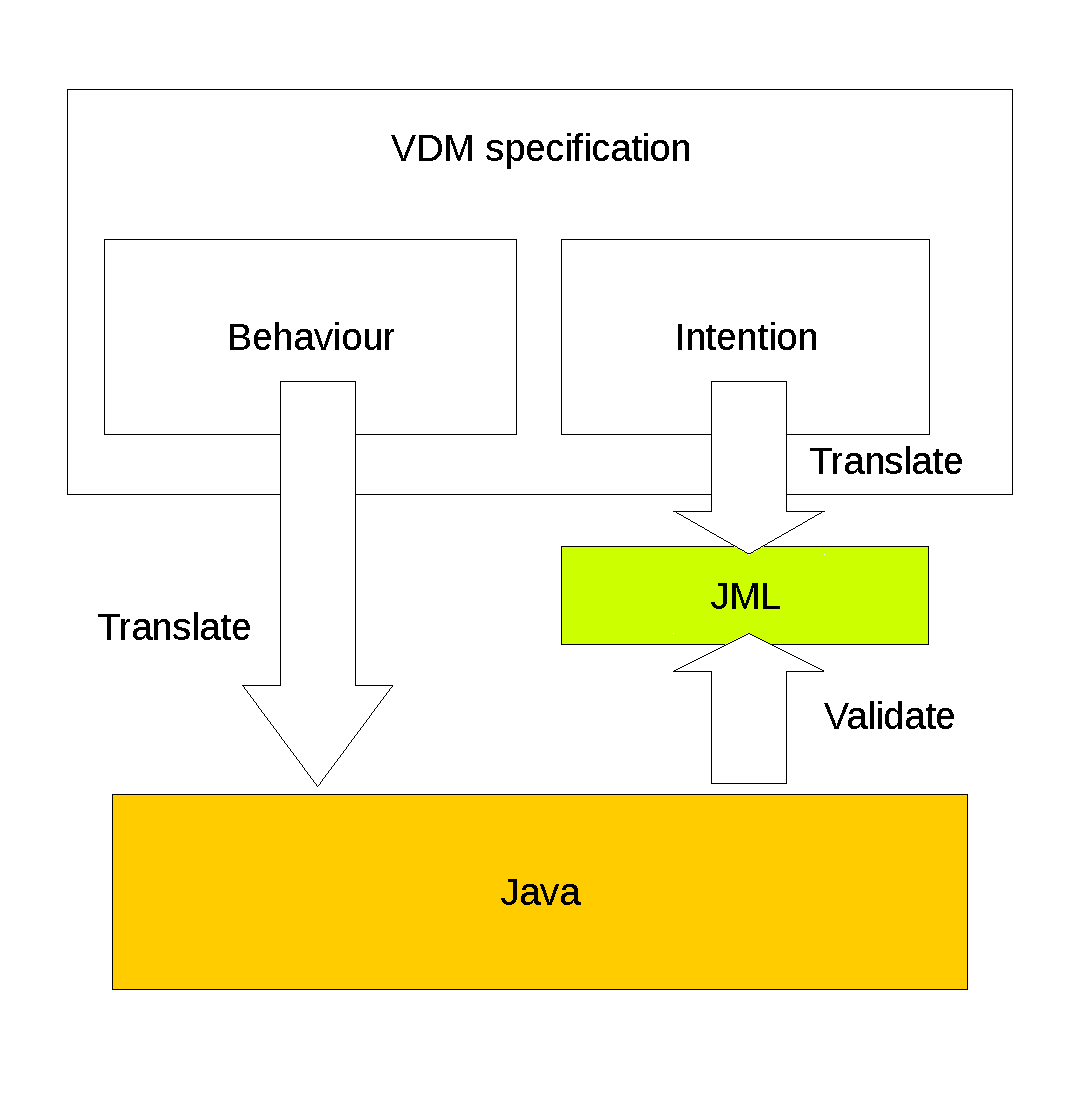
\includegraphics[width=0.6\linewidth]{figs/vdm2jml}
  \caption {Overview of the \ac{vdm}-to-JML translation.}
  \label{fig:vdm2jml-overview}
\end{figure}

\subsection{Background}

The translation is defined as a set of rules that are implemented as
an extension of Overture \ac{vdm}-to-Java code
generator~\cite{Jorgensen&14a} to make the approach fully automated.

\subsection{Prerequisites}

\begin{itemize}
\item Mention OpenJML
\item Mention rules and VDM-to-JML paper
\item Mention Overture
\end{itemize}

%%% Local Variables:
%%% mode: latex
%%% TeX-master: "../vdm2jml-tr"
%%% End:


% Reset acronyms
\acresetall


\chapter{The Translation}
\label{chp:trans}


\chapter{Introduction}

A model specified using the \ac{vdm} can be validated against its
contract-based elements (e.g.\ pre and postconditions and invariants)
in order to ensure that the system behaves as intended. One way to
validate the model against its contracts is by animation using
Overture's \ac{vdm} interpreter.

When sufficient insight into the system under development has been
obtained during the formal analysis, development proceeds to the
implementation phase, where the system is realised. One way to realise
a \ac{vdm} model is by implementing it in a programming language, for
example, using code generation. However, since no guarantees are made
about the correctness of the generated code, other measures must be
taken to increase the confidence in the correctness of the generated
code.

To support this approach, Overture enables fully automated translation
of \vsl's contract-based elements (pre- and postconditions, and
invariants) and type constraints to \ac{jml} annotations. The \ac{jml}
generator is developed as an extension of Overture's \ac{vdm}-to-Java
code generator and produces \ac{jml} annotated Java programs. In this
way \ac{jml} tools can be used to validate the generated Java code
against the \emph{intended} system behaviour, described using
\ac{jml}. This work-flow is illustrated in
\cref{fig:vdm2jml-overview}.

\begin{figure}[!ht]
  \centering
  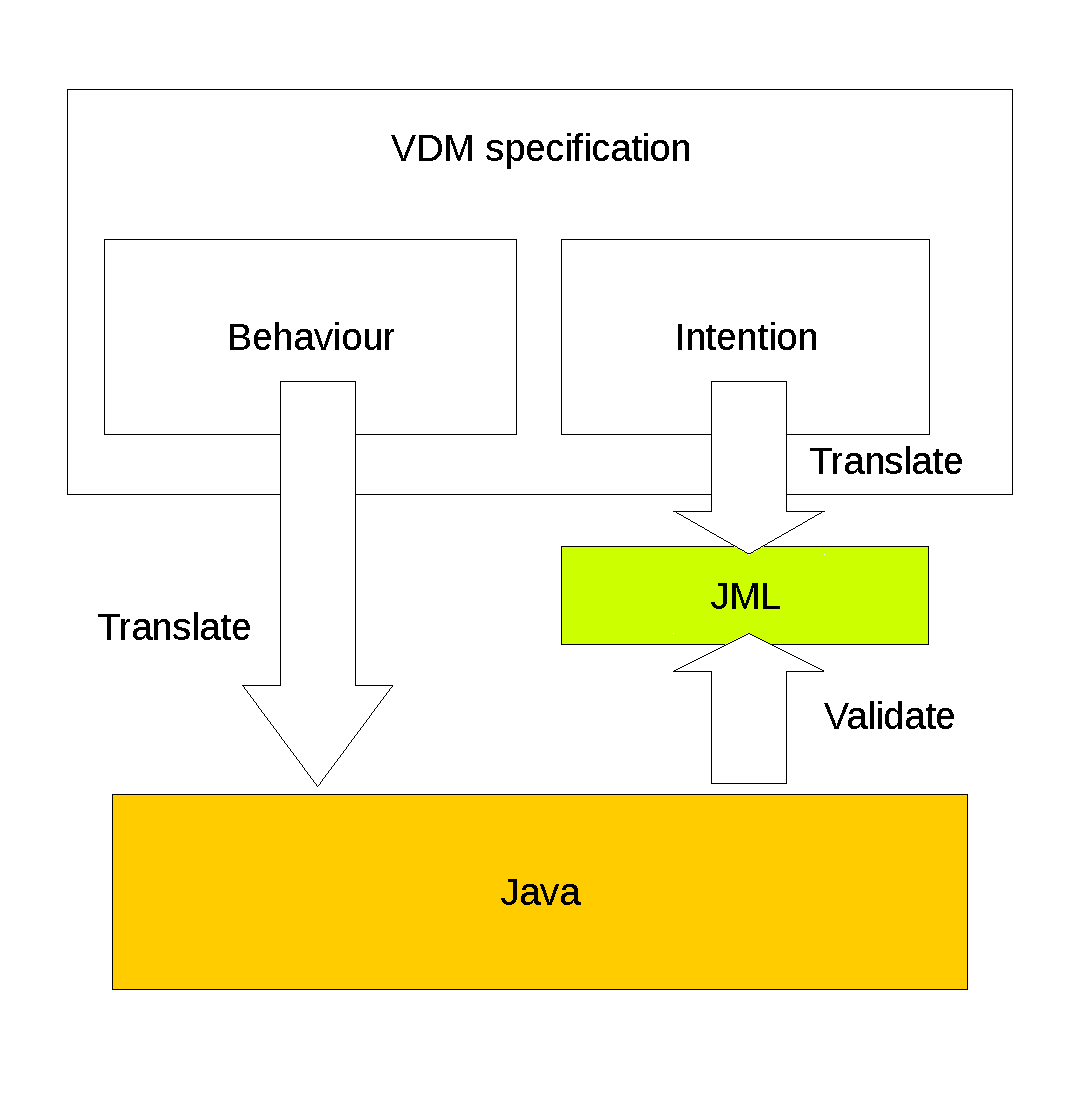
\includegraphics[width=0.6\linewidth]{figs/vdm2jml}
  \caption {Overview of the \ac{vdm}-to-JML translation.}
  \label{fig:vdm2jml-overview}
\end{figure}

\subsection{Background}

The translation is defined as a set of rules that are implemented as
an extension of Overture \ac{vdm}-to-Java code
generator~\cite{Jorgensen&14a} to make the approach fully automated.

\subsection{Prerequisites}

\begin{itemize}
\item Mention OpenJML
\item Mention rules and VDM-to-JML paper
\item Mention Overture
\end{itemize}

%%% Local Variables:
%%% mode: latex
%%% TeX-master: "../vdm2jml-tr"
%%% End:

\section{\ac{dbc} with \ac{vdmsl} and \ac{jml}}
\label{sec:vdmjml}

In this section we describe \ac{vdmsl} and \ac{jml}. We cover
different types and all the contract-based elements of \ac{vdmsl},
focusing specifically on the \ac{vdm}-10 release, which we are
targeting in our work. The \ac{jml} constructs described in this
section cover those that are used to implement the translation rules.

\subsection{\ac{vdmsl}}
\label{sub:vdmsl}

\ac{vdmsl} is an ISO standardised sequential modelling language that
supports description of data and functionality. The ISO standard has
later been informally extended with modules to allow type definitions,
values (constants) and functionality to be imported and exported
between modules. A module may define a single state component, which
can be constrained by a state invariant. State is modified by
assigning a new value to a state designator, which can be either a
name, a field reference or a map or sequence reference, as described
in the \ac{vdm} language reference manual~\cite{Larsen&10b}.

Module state, if specified, implicitly defines a record type, which is
tagged with the state name and also defines the type of the state
component. The state type can be used like any other record type
explicitly defined by the modeller -- the difference being that the
state invariant~\cite{Andrews&98} constrains the state type and thus
every instance of this record type.

Data are defined by means of built-in basic types covering, for
instance, numbers, booleans, quote types and characters. A quote type
corresponds to an enumerated type in a language such as Pascal. The
basic types can be used to form new structured data types using
built-in type constructors that support creation of union types, tuple
types and record types. A type may also be declared optional, which
allows \kw{nil} to be used to represent the absence of a value. For
collections of values, \ac{vdmsl} supports sets, sequences and
maps. The built-in data types, type constructors and collections can
be used to form named user defined types, which can be constrained by
invariants. We refer to these types as \emph{named invariant
  types}. As an example, \autoref{lst:vdmAmount} shows the definition
of the named invariant type \texttt{Amount}, which is used to
represent an amount of money deposited or withdrawn by an account
holder. This type is defined based on natural numbers (excluding
zero), i.e.\ the built-in basic type \kw{nat1} in \ac{vdmsl}. For this
particular example, we say that \kw{nat1} is the \emph{domain type} of
\texttt{Amount}. We further constrain \texttt{Amount} using an
invariant, by requiring a value of this type to be less than
2000. Specifically, for the invariant shown in
\autoref{lst:vdmAmount}, the \texttt{a} on the left-hand side of the
equality is a pattern that matches values of type
\texttt{Amount}. This pattern is used to express the invariant
predicate for this named invariant type.

\begin{vdmsl}[style=customVdm,caption={Example of a \ac{vdmsl} named invariant type.},label={lst:vdmAmount}]
types
Amount = nat1
inv a == a < 2000;
\end{vdmsl}

\subsubsection{Functional descriptions}
\label{sec:functional-descriptions}

In \ac{vdm}, functionality can be defined in terms of functions and
operations over data types with a traditional call-by-value semantics.
Functions are referentially transparent and therefore they are not
allowed to access or manipulate state directly, whereas operations
are. Therefore, a function cannot call an operation.\footnote{With the
  recent introduction of \kw{pure} operations into \ac{vdm}-10 (not to
  be confused with \kw{pure} methods in \ac{jml}) it has become
  possible to invoke operations, albeit \kw{pure} ones, from a
  function. This feature was introduced to address issues with the
  object-oriented dialect of \ac{vdm}, called \ac{vdm}++, but was made
  available in every \ac{vdm}-10 dialect (including \ac{vdmsl}).} In
addition to accessing module state, operations may also use the
\kw{dcl} statement to declare local state designators which can be
assigned to. Subsequently the term \emph{functional description} will
be used to refer to both functions and operations. As an example, a
function that uses the \texttt{MATH`sqrt} library function to
calculate the square root of a real number is shown in
\autoref{lst:vdmSqrt}.

\begin{vdmsl}[style=customVdm,caption={\ac{vdmsl} function for
calculating the square root of a number.},label={lst:vdmSqrt}]
sqrt :  real -> real
sqrt (x) == MATH`sqrt(x)
pre x >= 0
post RESULT * RESULT = x;
\end{vdmsl}

Functional descriptions can be implicitly defined in terms of pre- and
postconditions, which specify conditions that must hold before and
after invoking the functional description. Alternatively, a functional
description can be \emph{explicitly} defined by means of an algorithm,
as shown in \autoref{lst:vdmSqrt}. The \ac{jml} translator supports
both implicitly and explicitly defined functional
descriptions. However, only methods that originate from explicitly
defined functional descriptions can be executed.

The precondition of a function can refer to all the arguments of the
function it guards. The same applies to the postcondition of a
function, which can also refer to the result of the execution using
the reserved word \kw{RESULT}. For the square root function in
\autoref{lst:vdmSqrt} we require that the input is a positive number
(the precondition), and that the square of the function result equals
the input value (the postcondition).

Function definitions are derived for the pre- and postconditions of
\texttt{sqrt} from \texttt{sqrt}'s \kw{pre} and \kw{post}
clauses. These function definitions do not appear in the model, but
they are used internally by the Overture interpreter to check for
contract violations. However, to clarify, the pre- and postcondition
functions of \texttt{sqrt} are shown in
\autoref{lst:vdmFuncPrePost}. In this listing, \texttt{+>} specifies
that \texttt{pre\_sqrt} and \texttt{post\_sqrt} are total functions,
and not partial functions, which use the \texttt{->} type constructor.

\begin{vdmsl}[style=customVdm,caption={Pre- and postcondition
functions for the \texttt{sqrt} function shown in
\autoref{lst:vdmSqrt}.},label={lst:vdmFuncPrePost}]
pre_sqrt:real +> bool
pre_sqrt(x) == x >= 0;

post_sqrt:real*real +> bool
post_sqrt(x,RESULT) == RESULT * RESULT = x;
\end{vdmsl}

Similarly, the pre- and postcondition functions of an operation are
also derived. To demonstrate this, consider the \texttt{inc} operation
in \autoref{lst:vdmInc}. This operation takes a real number as input,
adds it to a counter (defined using a state designator), and returns
the new counter value. In this listing \texttt{counter\~} and
\texttt{counter} refer to the counter values before and after the
operation has been invoked, respectively.

\begin{vdmsl}[style=customVdm,caption={\ac{vdmsl} operation for
incrementing a counter.},label={lst:vdmInc}]
inc : real ==> real
inc (i) == (
 counter := counter + i;
 return counter;
)
pre i > 0
post counter = counter~ + i and
     RESULT = counter;
\end{vdmsl}

A precondition of an operation can refer to the state, \texttt{s},
before executing the operation, whereas the postcondition of an
operation can read both the before and after states. State access is
achieved by passing copies of the state to the pre- and postcondition
functions. The corresponding pre- and postcondition functions for
\texttt{inc} are shown in \autoref{lst:vdmOpPrePost} where the
parameters \texttt{s\~} and \texttt{s} of \texttt{post\_inc} refer to
the state (that contains the counter value) before and after execution
of \texttt{inc}. We further use \texttt{S} to denote the record type
that represents the module's state.

\begin{vdmsl}[style=customVdm,caption={Pre- and postcondition
functions for the \texttt{inc} operation shown in
\autoref{lst:vdmInc}.},label={lst:vdmOpPrePost}]
pre_inc:real*S +> bool
pre_inc(i,s) == i > 0;

post_inc:real*real*S*S +> bool
post_inc(i,RESULT,s~,s) ==
s.counter = s~.counter + i and
RESULT = s.counter;
\end{vdmsl}

The function descriptions in \autoref{lst:vdmOpPrePost} assume that
the pre- and postconditions are defined (using the \kw{pre} and
\kw{post} clauses) and that the state of the module enclosing the
functional description exists. For the cases where pre- and
postconditions are not defined they can be thought of as functions
that yield \kw{true} for every input. Furthermore, when no state
component is defined, the pre- and postcondition functions simply omit
the state parameters. Similarly, when an operation does not return a
result (it specifies void as the return type) the postcondition
function omits the \kw{RESULT} parameter.

For each type definition constrained by an invariant, such as
\texttt{Amount} shown in \autoref{lst:vdmAmount}, a function is
implicitly created to represent the invariant -- see
\autoref{lst:vdmTypeInv}. The Overture tool uses this function
internally to check whether a value is consistent with respect to a
given type (e.g.\ \texttt{Amount})~\cite{Lausdahl&11}. Note that since
all invariants are functions they are not allowed to depend on state
of other modules. Specifically, invariants can only invoke functions
and access global constants (possibly defined in other modules).

\begin{vdmsl}[style=customVdm,caption={Invariant function for type
definition \texttt{Amount}.},label={lst:vdmTypeInv}]
inv_Amount : Amount +> bool
inv_Amount (a) == a < 2000;
\end{vdmsl}

\subsubsection{Atomic execution}

Multiple consecutive statements are sometimes needed to update the
state designators to make them consistent with the system's
invariants. For example, assume that we have a system that uses two
state designators called \texttt{evenID\sub{1}} and
\texttt{evenID\sub{2}} to store even and different numbers. For this
example, we will assume that these state designators are of type
\texttt{Even} -- a type that constrains these state designators to
store even numbers. To help ensure that the uniqueness constraint (a
state invariant) is not violated during an update, multiple
assignments can be grouped in an \kw{atomic} statement block as shown
in~\autoref{lst:vdmAtomic}. Given the type \texttt{Even} of the state designators
\texttt{evenID\sub{1}} and \texttt{evenID\sub{2}} it is as if the
atomic statement is evaluated as shown in \autoref{lst:vdmAtomicEval}.

\begin{vdmsl}[style=customVdm,caption={Atomic update in
\ac{vdm}.},label={lst:vdmAtomic}]
atomic (
 evenID!\sub{1}! := exp!\sub{1}!;
 evenID!\sub{2}! := exp!\sub{2}!;
)
\end{vdmsl}


\begin{vdmsl}[style=customVdm,caption={The execution semantics of the
\kw{atomic} statement.},label={lst:vdmAtomicEval}]
let t!\sub{1}! : Even = exp!\sub{1}!,
    t!\sub{2}! : Even = exp!\sub{2}!
in (
 -- Turn off invariants
 evenID!\sub{1}! := t!\sub{1}!;
 evenID!\sub{2}! := t!\sub{2}!;
 -- Turn on invariants
 -- Check invariants hold
);
\end{vdmsl}

Executing the \kw{atomic} statement block is semantically equivalent
to first evaluating the right-hand sides of all the assignments before
turning off invariant checks, and then binding the results to the
corresponding state designators. After all the assignments have been
executed, it must be ensured that all invariants hold.

There are three properties that follow from the evaluation semantics
of the \kw{atomic} statement block that are worth mentioning:

\begin{enumerate}

\item When evaluating the right-hand sides of the assignment
  statements, potential contract violations will be reported.

\item Temporary identifiers, used to store the right-hand side
  results, are explicitly typed and therefore violations of named
  invariant types for these variables will be reported. The explicit
  type annotations thus ensure that the right-hand side of a state
  designator assignment is checked to be consistent with the type of
  said state designator.

\item Assignment statements cannot see intermediate values of state
  designators.

\end{enumerate}

\subsection{\ac{jml}}
\label{sec:jml}

Although \ac{jml}~\cite{Leavens&13} is designed to specify arbitary
sequential Java programs, in this subsection we only describe the
features needed for the translation from \ac{vdmsl}.

A method specified with the \kw{pure} modifier in \ac{jml} is not
permitted to have write effects; such 
methods are allowed to be used in specifications. Pure methods are
used to translate \ac{vdmsl} functions.

A class invariant in \ac{jml} should hold whenever the non-helper
methods of that class are not being executed; thus invariants must
hold in each method's before and after states. However, a method
declared with the \kw{helper} annotation in a type \texttt{T} does not
have its pre- and postconditions augmented with \texttt{T}'s
invariants.  Helper methods (and constructors) must either be pure or
private~\cite{Leavens&13}, so that the invariant will hold at the
beginning and end of all client-visible
methods~\cite{Mueller-Poetzsch-Heffter-Leavens06}. The before and
after states of non-helper methods and constructors are said to be
\emph{visible states}; thus invariants must hold in all visible
states.  \ac{jml} distinguishes between instance and static
invariants. An \emph{instance} invariant can refer to the non-static
(i.e.\ instance) fields of an object.  A \emph{static\/} invariant
cannot refer to an object's non-static fields; thus static invariants
are used to specify properties of static fields.

An assertion can reference the invariant for an object explicity using
a predicate of the form \invariantfor{\texttt{(e)}}, which is
equivalent to the invariant for \texttt{e}'s static type \cite[section
12.4.22]{Leavens&13}.

In \ac{jml} pre- and postconditions are written using the keywords
\kw{requires} and \kw{ensures}, respectively. In the specification of
a postcondition, one writes \texttt{\textbackslash \textbf{old}(e)} to
refer to the before state value of an expression \texttt{e}.  For
example, an \texttt{increment} method that writes a field
\texttt{count} could be specified as shown in
\autoref{lst:jmlCounMethod}.

\begin{lstlisting}[style=customJml,label={lst:jmlCounMethod},caption={Example of a \ac{jml} specification for a Java method.}]
//@ requires count < Integer.MAX_VALUE;
//@ modifies count;
//@ ensures count == \old(count)+1;
void increment() {
  count++;
}
\end{lstlisting}
Method postconditions may also use the keyword {\RESULT} to refer to
the value returned by the method.

Specification expressions in \ac{jml} can use Java expressions that
are pure (have no write effects), and also some logical operators,
such as implication \texttt{==>}, and quantifiers such as {\JMLforall}
and {\JMLexists}.

In addition to method pre- and postconditions, one can also write
assertions anywhere a Java statement can appear, using \ac{jml}'s
\kw{assert} keyword. Such assertions must hold whenever they are executed.

One way to specify the abstract state of a class is to use \ac{jml}'s
\kw{ghost} variables. Ghost variables are specification-only variables
and fields of objects that can only be used in \ac{jml} specifications
and in \ac{jml} \kw{set} statements. A set statement is an assignment
statement whose target is a ghost variable.

By default, \ac{jml} variables and fields may not hold the \kw{null}
value. However, should one wish to specify that all fields of a class
may hold \kw{null}, then one can annotate the class's declaration with
\kw{nullable\_by\_default}.

%%% Local Variables: 
%%% mode: latex
%%% TeX-master: "../paper"
%%% End: 

\section{The implementation of the \ac{jml} translator}
\label{sec:sl2java}

The \ac{jml} translator is implemented as an extension to Overture's
\ac{vdmsl}-to-Java code-generator, which provides code-generation
support for a large executable subset of \ac{vdm}. This section
describes how the \ac{jml} translator has been implemented, and
explains the details of the Java code-generator that are needed in
order to understand how the \ac{jml} translator works.

\subsection{The implementation}

The Java code-generator is developed using Overture's code-generation
platform -- a framework for constructing code-generators for
\ac{vdm}~\cite{Jorgensen&14a}. This platform is used by the Java
code-generator to parse the \ac{vdmsl} model sources and to construct
an \ac{ir} of the model -- an \ac{ast} that constitutes an internal
representation of the generated code. The Java code-generator uses the
code-generation platform to \emph{transform} the \ac{ir} into a tree
structure that eventually is translated directly into Java code. The
translation of the \ac{ir} into Java is handled by the code-generation
platform's code emission framework, which uses the Apache Velocity
template engine~\cite{ApacheVelocity}.

The Java code-generator exposes the \ac{ir} during the code-generation
process, which allows the \ac{jml} translator to intercept the
code-generation process and further transform the \ac{ir}. These
additional transformations are used to decorate the \ac{ir} with nodes
that contain the \ac{jml} annotations. Using the code emission
framework, the final version of the \ac{ir} is translated into a
\ac{jml}-annotated Java program.

The \ac{jml} translator is publicly available in Overture version
2.3.8 (as of July 2016) onwards~\cite{Overture}. Furthermore, the
\ac{jml} translator's source code is available via the Overture tool's
open-source code repository~\cite{OvertureGithub}.

\subsection{Overview of the translation}

In the generated code, a module is represented using a \kw{final} Java
class with a \kw{private} constructor, since \ac{vdmsl} does not
support inheritance and a module cannot be instantiated. Due to the
latter, both operations and functions are code-generated as
\kw{static} Java methods.

Module state is represented using a \kw{static} class field in the
module class to ensure that only a single state component exists at
any given time. The state component is represented using a record
value, and as a consequence, an additional record type is 
generated to represent it.

Each variable in \ac{vdmsl} is passed by value, i.e.\ as a \emph{deep
  copy}, when it is passed as an argument, appears on the right-hand
side of an assignment or is returned as a result. As a consequence,
aliasing can never occur in a \ac{vdmsl} model. Types are different in
Java, where objects are modified via object references or
pointers. Therefore different object references can be used to modify
the same object. To avoid such aliasing in the generated code, data
types are code-generated with functionality to support value type
behaviour.

Every record definition code-generates to a class definition with
accessor methods for reading and manipulating the fields. This class
implements \texttt{equals} and \texttt{copy} methods to support
comparison based on structural equivalence and deep copying,
respectively. In this way the call-by-value semantics of \ac{vdmsl}
can be preserved in the generated code by invoking the \texttt{copy}
method, which helps to prevent aliasing. Similarly the \texttt{equals}
method can be invoked to compare code-generated records based on
structural equivalence rather than comparing addresses of object
references. A record object can then be obtained by invoking the
constructor of the record class or by invoking the \texttt{copy}
method of an existing record object.

Java does not support the definition of aliases of existing types,
such as the \texttt{Amount} named invariant type
in~\autoref{lst:vdmAmount}. Therefore, the Java code-generator chooses
not to code-generate class definitions for these types. Instead, a use of
a named invariant type is replaced with its domain type (described
in \autoref{sub:vdmsl}). Since the named invariant type is an alias of
an existing type this is fine, as long as we make sure to check that
the type invariant holds.

% [I think the following may be more natural for Java -- Gary]
% [Yes you can argue that, but there are other (good) reasons for not doing it. I omitted this paragraph as I don't want the paper to get into a discussion about this -- Peter TJ]
% Alternatively, the Java code-generator could have generated a class
% definition to represent the named invariant type directly. As a
% consequence of the current approach fewer class definitions are
% generated. However, as we shall see in~\autoref{sec:sl-other-gen},
% this approach imposes some different challenges to the translation of
% named invariant types to \ac{jml} compared to that of translating
% state invariants.

To assist the translation of \ac{vdm} to Java, the existing Java
code-generator uses a runtime library, which among other things,
includes Java implementations for some of the different \ac{vdm} types
and operators. The \texttt{Tuple} class, for example, is used to
represent tuple types and enables construction of tuple values. Sets,
sequences and maps are represented using the \texttt{VDMSet},
\texttt{VDMSeq} and \texttt{VDMMap} classes, which themselves are
based on Java collections, and so on. The runtime library's collection
classes are used as raw types (e.g.\ \texttt{VDMSet}) in the generated
code, and therefore they are never passed a generic type argument. Raw
types provide a convenient way to represent \ac{vdm} collections that
store elements of some union type -- a kind of type that Java does not
support.

In addition to using the existing runtime library, the \ac{jml}
translator also contributes a small runtime library to aid the
generation of \ac{jml} checks. This runtime library, which we
subsequently refer to as \texttt{V2J}, is an extension of the existing
Java code-generator runtime library. As we shall see in
\autoref{sec:col}, the \texttt{V2J} runtime is mostly used in the
generated \ac{jml} checks to ensure that instances of collections
respect the \ac{vdm} types that produce them.


%%% Local Variables:
%%% mode: latex
%%% TeX-master: "../../vdm2jml-tr"
%%% End:

\section{Case study example}
\label{sec:case}

Throughout the report we will demonstrate the translation rules using a
case study model of an \ac{atm}. The model consists of a single
module, \texttt{ATM} (shown in \autoref{lst:vdmCase}), which uses a
state definition to record information about

\begin{itemize}

\item The debit cards considered valid by the system (named
  \texttt{validCards}).

\item The debit card currently inserted into the \ac{atm}, if any
  (\texttt{currentCard}).

\item If a valid PIN code has been entered (\texttt{pinOk}) for the
  debit card currently inserted into the \ac{atm} and,

\item all the bank accounts known to the system (\texttt{accounts}).

\end{itemize}

\begin{vdmsl}[style=customVdm,caption={\ac{vdmsl} module representing
an \ac{atm}.},label={lst:vdmCase}]
module ATM
definitions
state St of
 validCards : set of Card
 currentCard : [Card]
 pinOk : bool
 accounts : map AccountId to Account
 init St == St = @mk_@St({},nil,false,{|->})
 inv @mk_@St(v,c,p,a) ==
  (p or c <> nil => c in set v)
  and
  forall id1, id2 in set dom a &
   id1 <> id2 =>
   a(id1).cards inter a(id2).cards = {}
end
 ...
operations
GetStatus : () ==> bool * seq of char
GetStatus () == ...

OpenAccount : set of Card * AccountId ==> ()
OpenAccount (cards,id) == ...

AddCard : Card ==> ()
AddCard (c) == ...

RemoveCard : Card ==> ()
RemoveCard (c) == ...

InsertCard : Card ==>
  <Accept>|<Busy>|<Reject>  
InsertCard (c) == ...

EnterPin : Pin ==> ()
EnterPin (pin) == ...

ReturnCard : () ==> ()
ReturnCard () == ...

Withdraw : AccountId * Amount ==> real
Withdraw (id, amount) == ...

Deposit : AccountId * Amount ==> real
Deposit (id, amount) == ...
end
\end{vdmsl}

For simplicity, \autoref{lst:vdmCase} omits type definitions and only
shows the state definition (including the state invariant) and the
signatures for some of the operations. The state invariant, shown in
\autoref{lst:vdmCase}, requires that at all times the following two
conditions must be met: a debit card must at most be associated with a
single account and secondly, for a PIN code to be considered valid,
the debit card currently inserted into the \ac{atm} must itself be a
valid debit card.

When the \ac{atm} model is translated to a \ac{jml}-annotated Java
program it can be checked for correctness using \ac{jml} tools. To
demonstrate this, consider the example in \autoref{lst:jmlScenario},
which creates a debit card, inserts it into the \ac{atm}, and performs
a transaction scenario.

\begin{lstlisting}[style=customJml,caption={Java code demonstrating
use of the implementation of the \ac{atm}
model.},label={lst:jmlScenario}]
Card c = new Card(5,1234);
// atm.ATM.AddCard(c); (missing statement)
atm.ATM.InsertCard(c);
atm.ATM.EnterPin(1234);
System.out.println(atm.ATM.GetStatus());
/* Transaction related code omitted */
atm.ATM.ReturnCard();
\end{lstlisting}

If this program is executed using the OpenJML runtime assertion
checker the output in \autoref{lst:racOutput} is reported.

\begin{lstlisting}[style=racOutput,caption={Inconsistent use of the
system detected using the OpenJML runtime assertion
checker.},label={lst:racOutput}]
Exception in thread "main" java.lang.AssertionError: Main.java:12: JML precondition is false
        atm.ATM.EnterPin(1234);
                        ^
atm/ATM.java:276: Associated declaration: Main.java:12: 
  //@ requires pre_EnterPin(pin,St);
      ^
	at Main.main(Main.java:17)
\end{lstlisting}

For this particular example, this error is reported because the debit
card \texttt{c} is not recognised as a valid debit card by the
system. More specifically, the scenario did not invoke
\texttt{atm.ATM.AddCard(c)} immediately after creating the debit
card. The return value of the \texttt{Insert} method did indicate that
the debit card was rejected, but this value was mistakenly discarded
in \autoref{lst:jmlScenario}. The error is reported by the runtime
assertion checker because entering a PIN code when no debit card is
inserted into the \ac{atm} is considered an error. After changing the
example in \autoref{lst:jmlScenario} to add \texttt{c} as a valid
debit card, no problems are detected by the runtime assertion checker,
as expected. Therefore, the code executes as if it was compiled using
a standard Java compiler and executed on a regular Java virtual
machine. More, specifically, the system will report the status as
shown in \autoref{lst:racOutputSuccess} to indicate that the \ac{atm}
is not awaiting a debit card, and that a transaction is in progress.

\begin{lstlisting}[style=racOutput,caption={System output after fixing
the problem in
\autoref{lst:jmlScenario}.},label={lst:racOutputSuccess}]
mk_(false, "transaction in progress.")
\end{lstlisting}

As we proceed, in \autoref{sec:sl-dbc-gen} and
\autoref{sec:sl-types-gen} we elaborate on the specifics of each
\ac{vdm} definition in the case study model and demonstrate the
translation to \ac{jml}-annotated Java.


%%% Local Variables:
%%% mode: latex
%%% TeX-master: "../../vdm2jml-tr"
%%% End:

\section{Translating \ac{vdmsl} contracts to \ac{jml}}
\label{sec:sl-dbc-gen}

In this section we present the rules used to translate the \ac{dbc}
elements of \ac{vdmsl} to \ac{jml} annotations that are added to the
generated Java code. For each of the elements, we describe the
approach used to translate the element to \ac{jml}. This is afterwards
generalised as a rule, which appears in a grey box.

\subsection{Allowing null values by default}
\label{sec:modules}

Overture's Java code-generator may sometimes introduce auxiliary
variables that are initialised to \kw{null} when it code-generates
some of the constructs of \ac{vdm}. To avoid having errors reported
when checking the generated code with a \ac{jml} tool, we allow
\kw{null} as a legal value by default for all references in the
generated code.

\transRule{Allowing null values by default} {Annotate every class output by the
  Java code-generator with the \kw{nullable\_by\_default} modifier to
  allow all references to use \kw{null} as a legal value.}
%
\newcounter{nullRule}
\setcounter{nullRule}{\arabic{transRule}}
%

As a consequence we also have to guard against \kw{null} values for
variables that originate from \ac{vdm} variables or
patterns\footnote{The generated code uses variables to represent the
  patterns (record pattern, tuple pattern, identifier pattern etc.)
  introduced by use of pattern matching in \ac{vdm}.}  that do not
allow \kw{nil}.

\subsection{Translating functional descriptions to \ac{jml}}
\label{sec:func-desc}

Recall that a \ac{vdmsl} function code-generates to a \kw{static} Java
method. In addition, a \ac{vdmsl} function does not have side-effects
and therefore the code-generated version of the method can be
annotated as \ac{jml} \kw{pure}.

\transRule{Translation of functions}{Any function -- whether it is
  defined by the user or derived, e.g.\ from a \kw{pre} or \kw{post}
  condition clause -- code-generates to a \kw{static} Java method that
  is annotated with the \kw{pure} modifier.}
%
\newcounter{funcRule}
\setcounter{funcRule}{\arabic{transRule}}
%

Operations, on the other hand, can read and manipulate the state of
the enclosing module, or invoke other operations that may have
side-effects. Therefore, the method that the operation code-generates
to cannot be annotated as \ac{jml} \kw{pure}.

When a \ac{vdmsl} definition (e.g.\ a functional description) is
code-generated to Java, the visibility of the corresponding Java
definition can, in principle, be set according to whether the
\ac{vdmsl} definition is exported (\kw{public}) or not
(\kw{private}). In the presentation of the translation rules following
this section, we omit explicit use of access specifiers in the rule
formulation as we do not consider it crucial to our work.

\subsection{Translating preconditions to \ac{jml}}

In terms of semantics there is no difference between a precondition in
\ac{vdmsl} and \ac{jml}. There are, however, interesting issues worth
mentioning regarding how the \ac{jml} translator implements the
translation. We start by covering preconditions of operations, and we
end this subsection by describing how they differ from those of
functions. As an example of how a \ac{vdmsl} precondition is
translated, consider the operation
in~\autoref{lst:vdmWithdrawPre}. This operation models withdrawal from
a bank account identified by the parameter \texttt{id}.

\begin{vdmsl}[style=customVdm,caption={\ac{vdmsl} operation for bank
account withdrawal guarded by a precondition.},label={lst:vdmWithdrawPre}]
Withdraw : AccountId * Amount ==> real
Withdraw (id, amount) ==
let newBalance =
    accounts(id).balance - amount
in (
 accounts(id).balance := newBalance;
 return newBalance;
)
pre
currentCard in set validCards and pinOk and
currentCard in set accounts(id).cards and
id in set dom accounts
\end{vdmsl}

In order to withdraw money from the account, we require that a valid
card has been inserted, the PIN code is accepted, and that the bank
account exists. Note that since \texttt{currentCard} is of the
optional type \texttt{[Card]} it can be \kw{nil}, which is not a valid
member of \texttt{validCards}. Therefore, the precondition is
\kw{false} when no debit card has been inserted into the \ac{atm}. The
\texttt{pre\_Withdraw} function, which is not a visible part of the
model, is derived from the \kw{pre} clause of the \texttt{Withdraw}
operation. In the generated code this function is represented using a
\kw{pure} method according to rule \arabic{funcRule} -- see
\autoref{lst:jmlPreWithdraw}. Note that for the method in
\autoref{lst:jmlPreWithdraw}, the Java code-generator uses extra
variables to perform the equivalent \ac{vdm} computation. These extra
variables are also type checked using \ac{jml} (although they are only
used to store intermediate results).

\begin{lstlisting}[float=*,style=customJml,caption={Code-generated version of
the \texttt{pre\_Withdraw} operation.},label={lst:jmlPreWithdraw}]
/*@ pure @*/
public static Boolean pre_Withdraw(
    final Number id, final Number amount, final atm.ATMtypes.St St) {
  //@ assert (Utils.is_nat(id) && inv_ATM_AccountId(id));
  //@ assert (Utils.is_nat1(amount) && inv_ATM_Amount(amount));
  //@ assert Utils.is_(St,atm.ATMtypes.St.class);
  Boolean andResult_3 = false;
  //@ assert Utils.is_bool(andResult_3);
  if (SetUtil.inSet(St.get_currentCard(), St.get_validCards())) {
    Boolean andResult_4 = false;
    //@ assert Utils.is_bool(andResult_4);
    if (St.get_pinOk()) {
      Boolean andResult_5 = false;
      //@ assert Utils.is_bool(andResult_5);
      if (SetUtil.inSet(St.get_currentCard(),
          ((atm.ATMtypes.Account) Utils.get(St.accounts, id)).get_cards())) {
        if (SetUtil.inSet(id, MapUtil.dom(St.get_accounts()))) {
          andResult_5 = true;
          //@ assert Utils.is_bool(andResult_5);
        }
      }
      if (andResult_5) {
        andResult_4 = true;
        //@ assert Utils.is_bool(andResult_4);
      }
    }
    if (andResult_4) {
      andResult_3 = true;
      //@ assert Utils.is_bool(andResult_3);
    }
  }
  Boolean ret_29 = andResult_3;
  //@ assert Utils.is_bool(ret_29);
  return ret_29;
}
\end{lstlisting}

The \texttt{Withdraw} operation is translated to the method shown
in~\autoref{lst:jmlWithdraw}. This method introduces several \ac{jml}
assertions that will be described in \autoref{sec:sl-types-gen}. Note
that the \texttt{pre\_Withdraw} method is invoked from the
\kw{requires} clause of the \texttt{Withdraw} method to check whether
the precondition is met. In addition to the input parameters of the
\texttt{Withdraw} method, the \texttt{pre\_Withdraw} method is also
passed the state \texttt{St}.

\begin{lstlisting}[float=*,style=customJml,caption={Code-generated version of
the \texttt{Withdraw} operation.},label={lst:jmlWithdraw}]
//@ requires pre_Withdraw(id,amount,St);
public static Number Withdraw(final Number id, final Number amount) {
 //@ assert (Utils.is_nat(id) && inv_ATM_AccountId(id));
 //@ assert (Utils.is_nat1(amount) && inv_ATM_Amount(amount));
 final Number newBalance =
     ((atm.ATMtypes.Account) Utils.get(St.accounts, id)).get_balance().doubleValue()
         - amount.longValue();
 //@ assert Utils.is_real(newBalance);
 {
   VDMMap stateDes_1 = St.get_accounts();
   atm.ATMtypes.Account stateDes_2 = ((atm.ATMtypes.Account) Utils.get(stateDes_1, id));
   //@ assert stateDes_2 != null;
   stateDes_2.set_balance(newBalance);
   //@ assert (V2J.isMap(stateDes_1) && (\forall int i; 0 <= i && i < V2J.size(stateDes_1); (Utils.is_nat(V2J.getDom(stateDes_1,i)) && inv_ATM_AccountId(V2J.getDom(stateDes_1,i))) && Utils.is_(V2J.getRng(stateDes_1,i),atm.ATMtypes.Account.class)));
   //@ assert Utils.is_(St,atm.ATMtypes.St.class);
   //@ assert \invariant_for(St);
   Number ret_7 = newBalance;
   //@ assert Utils.is_real(ret_7);
   return ret_7;
 }
}
\end{lstlisting}

\transRule{Translating the precondition of an operation} {
  Let \texttt{op} be a method code-generated from a \ac{vdmsl} user-defined operation and let the signature of \texttt{op} be:\\
  \kw{static} \texttt{R op(I\sub{1} i\sub{1},...,I\sub{n} i\sub{n})}\\
  Then \texttt{op} has a code-generated precondition method\\
  \texttt{pre\_op} that is \kw{pure} and which in addition to the
  pa\-ra\-met\-ers of \texttt{op} also takes the state component \texttt{s} as an argument, i.e.\ \\
  \texttt{/*@ \kw{pure} @*/} \kw{static} \texttt{ \kw{boolean}\\
    pre\_op(I\sub{1} i\sub{1},...,I\sub{n} i\sub{n},S s)}\\
  To ensure that the precondition is evaluated, we annotate \texttt{op} with the following \kw{requires} annotation:\\
  \texttt{//@ \kw{requires} pre\_op(i\sub{1},...,i\sub{n},s);}}
%
\newcounter{preOp}
\setcounter{preOp}{\arabic{transRule}}
%
Rule \arabic{preOp} assumes the existence of a state component
\texttt{s}. However, when the state of the module enclosing
\texttt{op} is not defined, rule \arabic{preOp} changes to not include
the state parameter in the definition of \texttt{pre\_op}.

The example above considers the case where the precondition is
guarding an operation (i.e.\ \texttt{Withdraw}). As described in
\autoref{sec:vdmjml}, a precondition is defined differently for a
function than it is for an operation. In particular, the precondition
of a function is not passed the state, so neither is the
code-generated version of it. We also note that the visibility of the
precondition function must be the same as that of the functional
description it guards. Otherwise it cannot be invoked from the
corresponding \kw{requires} clause.

\transRule{Translating the precondition of a function} {
  Let \texttt{f} be a method code-generated from a \ac{vdmsl} user-defined function and let the signature of \texttt{f} be:\\
  \kw{static} \texttt{R f(I\sub{1} i\sub{1},...,I\sub{n} i\sub{n})}\\
  Then \texttt{f} has a code-generated precondition method
  \texttt{pre\_f} that is \kw{pure} and which accepts the same parameters as \texttt{f}, i.e.\ \\
  \texttt{/*@ \kw{pure} @*/} \kw{static} \texttt{ \kw{boolean}\\
    pre\_f(I\sub{1} i\sub{1},...,I\sub{n} i\sub{n})}\\
  To ensure that the precondition is evaluated, we annotate \texttt{f} with the following \kw{requires} annotation:\\
  \texttt{//@ \kw{requires} pre\_f(i\sub{1},...,i\sub{n});}}
  
\subsection{Translating postconditions to \ac{jml}}
\label{sec:postcond}

Postconditions in \ac{vdmsl} and \ac{jml} are semantically similar,
although \ac{vdmsl} represents the postcondition function as a derived
function definition (as was done for preconditions). Furthermore, in
\ac{vdm} and \ac{jml} postconditions of operations and methods,
respectively, can access both the before and after states. Returning
to the \texttt{Withdraw} operation, one could specify a postcondition
requiring that exactly the value specified by the \texttt{amount}
parameter is withdrawn from the account -- see
~\autoref{lst:vdmWithdrawPost}.

\begin{vdmsl}[style=customVdm,caption={The \texttt{Withdraw} operation
guarded by a postcondition.},label={lst:vdmWithdrawPost}]
Withdraw : AccountId * Amount ==> real
Withdraw (id, amount) == ...
post
let accountPre = accounts~(id),
    accountPost = accounts(id)
in
 accountPre.balance =
 accountPost.balance + amount and
 accountPost.balance = RESULT;
\end{vdmsl}

The JML translator produces a \kw{pure} Java method to represent the
postcondition function. This Java method is invoked from the
\kw{ensures} clause to check that the postcondition holds. The
invocation of the postcondition method of the \texttt{Withdraw}
operation is shown in~\autoref{lst:jmlWithdrawPost}.

\begin{lstlisting}[style=customJml,caption={Code-generated version of
the \texttt{Withdraw} operation.},label={lst:jmlWithdrawPost}]
//@ requires pre_Withdraw(id,amount,St);
//@ ensures post_Withdraw(id,amount,\result,\old(St.copy()),St);
public static Number Withdraw(final Number id, final Number amount) {...}
\end{lstlisting}

Note in particular how the before and after states are passed to the
\texttt{post\_Withdraw} method. Reasoning about before state is
achieved using \ac{jml}'s \old expression. For the \texttt{Withdraw}
operation the before state is constructed as \oldexp{St.copy()}. Since
\texttt{St.copy()} is a deep copy of the state (as explained
in~\autoref{sec:sl2java}) the evaluation inside the \old expression
ensures that the result indeed is a representation of the before
state.

The \ac{jml} translator deep copies the state because Java represents
every composite data type using a class. So without deep copying the
state, only the address of the before state object reference is
copied. In effect, only a single object would exist to represent the
pre- and post states. This would never work, since state changes made
by the operation would affect what was intended to be a representation
of the before state. Therefore, the state is deep copied to get a
separate object to represent the before state.

\transRule{Translating the postcondition of an operation} {
  Let \texttt{op} be a method code-generated from a \ac{vdmsl} user-defined operation and let the signature of \texttt{op} be:\\
  \kw{static} \texttt{R op(I\sub{1} i\sub{1},...,I\sub{n} i\sub{n})}\\
  Then \texttt{op} has a code-generated postcondition method\\
  \texttt{post\_op} that is \kw{pure} and which in addition to the
  parameters of \texttt{op}, also takes the result and the before and after states of \texttt{op} as arguments, i.e.\ \\
  \texttt{/*@ \kw{pure} @*/} \kw{static} \texttt{ \kw{boolean}}\\
  \texttt{ post\_op(I\sub{1} i\sub{1},...,I\sub{n} i\sub{n},}\\
  \indent \texttt{R RESULT,S \_s,S s)}\\
  To ensure that the postcondition is evaluated we annotate \texttt{op} with the following \kw{ensures} annotation:\\
  \texttt{//@ \kw{ensures}
    post\_op(i\sub{1},...,i\sub{n},\textbackslash\kw{result},}\\
  \indent \texttt{\textbackslash\textbf{old}(s.copy()),s);}}
%
\newcounter{postOp}
\setcounter{postOp}{\arabic{transRule}}
%

While the primary concern is to preserve the behaviour of the
specification across the translation, deep copying values may
significantly affect system performance in a negative way. In
particular, because it is difficult (in general) to avoid deep copying
values unnecessarily when they are passed around in the generated
code. To address this issue, the Java code-generator (and hence the
\ac{jml} translator) offers an option that, when selected by the user,
omits deep copying of values (other than the old state). While the
purpose of this is to generate performance-efficient code, this option
is, however, only safe to use if Java objects that originate from
\ac{vdmsl} values are not modified via aliases.

Yi et al.\ identify and address a number of problems with the \old
expression~\cite{Yi&2013}. In particular, the authors of that work
conduct experiments showing that passing deep copies of the old state
may drastically increase a system's memory usage. To address this, Yi
et al.\ propose the \past expression as a more memory-efficient
alternative to the \old expression. Yi et al.\ further show that the
\past expression can be implemented as an extension of the OpenJML
runtime assertion checker by means of aspect-oriented programming
principles. However, OpenJML does not officially support the \past
expression yet, which is why the translation rules do not currently
rely on this expression. As we see it, the ideas proposed by Yi et
al.\ could potentially support the development of a more
performance-efficient way to handle old states in the \ac{jml}
translator.

Similar to rule \arabic{preOp}, rule \arabic{postOp} also assumes that
the state of the module enclosing \texttt{op} exists. If the state
component does not exist, rule \arabic{postOp} changes to not include
the state parameters in the definition of
\texttt{post\_op}. Furthermore, if \texttt{op} does not return a
result (the return type is void), then the definition of
\texttt{post\_op} does not include the \texttt{RESULT} parameter.

The example above considers the postcondition of an operation (i.e.\
\texttt{Withdraw}). As described in \autoref{sec:vdmjml}, the
postcondition of a function is not allowed to access state. Therefore, the
code-generated version of the postcondition function is not
passed the state.

\transRule{Translating the postcondition of a function} {
  Let \texttt{f} be a method code-generated from a \ac{vdmsl} user-defined function and let the signature of \texttt{f} be:\\
  \kw{static} \texttt{R f(I\sub{1} i\sub{1},...,I\sub{n} i\sub{n})}\\
  Then \texttt{f} has a code-generated postcondition method\\
  \texttt{post\_f} that is \kw{pure} and which in addition to the
  parameters of \texttt{f} also takes the result of \texttt{f} as an argument, i.e.\ \\
  \texttt{/*@ \kw{pure} @*/} \kw{static} \texttt{ \kw{boolean}\\
    post\_f(I\sub{1} i\sub{1},...,I\sub{n} i\sub{n},R RESULT)}\\
  To ensure that the postcondition is evaluated we annotate \texttt{f} with the following \kw{ensures} annotation:\\
  \texttt{//@ \kw{ensures}
    post\_f(i\sub{1},...,i\sub{n},\textbackslash\kw{result});}}

\subsection{Translating record invariants to \ac{jml}}
\label{sub:rec-inv}

A record can, like any other type definition in \ac{vdmsl}, be
constrained by an invariant. As an example,~\autoref{lst:vdmRec} shows
a record definition modelling a bank account.

\begin{vdmsl}[style=customVdm,caption={A \ac{vdmsl} record definition
modelling a bank account.},label={lst:vdmRec}]
Account :: 
 cards : set of Card
 balance : real
 inv a == a.balance >= -1000;
\end{vdmsl}

An \texttt{Account} comprises the available balance as well as the
debit cards associated with the account. We further constrain an
\texttt{Account} to not have a balance of less than -1000, which is
expressed using an invariant.

As described in~\autoref{sec:sl2java}, a record definition is
translated to a class that emulates the behaviour of a value type
using \texttt{copy} and \texttt{equals} methods.

Since a record invariant is required to hold for every record value,
or object instance in the generated code, we represent it using an
\kw{instance invariant} in \ac{jml} as shown
in~\autoref{lst:jmlRec}. Note that the \kw{instance} \kw{invariant} is
formulated as an implication such that invariant violations are not
reported when invariant checks are disabled. As we shall see in
\autoref{sec:atomic} this has to do with the way \ac{vdmsl} handles
atomic execution.

% PJ: Make listing a float to avoid unintentional page-break

\begin{lstlisting}[float,style=customJml,caption={Code-generated version
of the \texttt{Account} record.},label={lst:jmlRec}]
//@ nullable_by_default
final public class Account implements Record
{
 public VDMSet cards;
 public Number balance;
 //@ public instance invariant atm.ATM.invChecksOn ==> inv_Account(cards,balance);
  ...
 /*@ pure @*/
 public boolean equals(final Object obj)
 {...}
 /*@ pure @*/
 public atm.ATMtypes.Account copy(){...}
 /*@ pure @*/
 public VDMSet get_cards() {...}
 public void set_cards(final VDMSet _cards)
 {...}
 /*@ pure @*/
 public Number get_balance() {...}
 public void set_balance(final Number _balance) {...}
 /*@ pure @*/
 /*@ helper @*/
 public static Boolean inv_Account(final VDMSet _cards, final Number _balance){
   return _balance.doubleValue() >= -1000L;
 }
}
\end{lstlisting}

The code-generated record \texttt{Account} defines an \emph{invariant
  method} \texttt{inv\_Account} that takes all the record fields of
\texttt{Account} as input and evaluates the invariant predicate. This
method is invoked directly from the \ac{jml} invariant, as shown in
\autoref{lst:jmlRec}. Note that \texttt{inv\_Account} is a \kw{static}
method according to rule \arabic{funcRule}. In addition, this
method is annotated as a \kw{helper} to avoid the invariant check
triggering another invariant check, which eventually would cause a
stack-overflow.

\transRule{Translating a record invariant}{Let \texttt{D} be a
  code-generated record definition with fields
  \texttt{f\sub{1},...,f\sub{n}} of types
  \texttt{F\sub{1},...,F\sub{n}}, respectively, and let \texttt{D} be
  constrained by an invariant. Then \texttt{D} has an invariant method
  \texttt{inv\_D} that is annotated as a \kw{helper} to allow it to
  be invoked from the invariant clause of \texttt{D}. The invariant
  method can also be annotated as \kw{pure} since it originates from a
  function definition. The annotated signature of \texttt{inv\_D} thus
  becomes:\\
  \texttt{/*@ \kw{pure} @*/}\\
  \texttt{/*@ \kw{helper} @*/}\\
  \kw{boolean} \texttt{inv\_D(F\sub{1} f\sub{1},...,F\sub{n} f\sub{n})}\\
  Let further \texttt{invChecksOn} be a variable that is true if
  invariant checking is enabled and false otherwise. To represent the
  record invariant of \texttt{D} we annotate \texttt{D} with the
  \kw{invariant} annotation:\\
  \texttt{/*@ \kw{public} \kw{instance} \kw{invariant}\\invChecksOn
    \kw{==>} inv\_D(f\sub{1},...,f\sub{n}); @*/}}

As we shall later see in \autoref{sec:atomic}, atomic execution
sometimes requires extra assertions to be inserted into the generated
code in order to guarantee that the record invariant semantics of
\ac{vdmsl} are preserved.

All the methods inside a record class -- except for the constructor
and the ``setter'' methods -- do not modify the state of the record
class and therefore they are marked as \kw{pure}. Updates to a record
object in the generated code are made using the ``setter'' methods of
the generated record class, or by using the record modification
expression~\cite{Larsen&10b}. Use of ``setter'' methods instead of
direct field access to manipulate the state of a record (which is how
field access is achieved in \ac{vdmsl}) forces the record object into
a \emph{visible state} (as described in \autoref{sec:jml}) after it
has been updated, thus triggering the invariant check according to
the \ac{vdmsl} semantics. For example, in \ac{vdmsl} we could set
the balance of an account as shown in \autoref{lst:vdmAccountUpdate}.

\begin{vdmsl}[style=customVdm,caption={Updating the \texttt{Account}
balance in \ac{vdmsl}.},label={lst:vdmAccountUpdate},numbers=none]
acc.balance := newBalance;
\end{vdmsl}

\noindent This assignment produces the Java code shown in
\autoref{lst:jmlAccountUpdate}. Note that for this particular case
there is no need to generate any additional \ac{jml} assertions since
the state of \texttt{acc} becomes visible after the call to
\texttt{set\_balance}. This causes the invariant check of
\texttt{Account} to trigger.

\begin{lstlisting}[style=customJml,caption={Updating the
\texttt{Account} balance in the generated
code.},label={lst:jmlAccountUpdate},numbers=none]
acc.set_balance(newBalance);
\end{lstlisting}

% In \ac{vdmsl} an invariant is a function, which means that it cannot
% call operations -- only calls to functions are
% allowed.\footnote{Recent changes to \ac{vdm}10 now allows \kw{pure}
%   operations (different from the \kw{pure} concept in \ac{jml}) to be
%   called from functions.}. Java, on the other hand, uses methods to
% express functionality, but it does not distinguish between functions
% and operations as \ac{vdm} does. Therefore every functional
% description in a \ac{vdmsl} model generates to a Java method.

%\todo[inline]{Re-consider this paragraph}

% The record invariant method (e.g.\ \texttt{inv\_Account}) is defined
% within the record class (e.g.\ \texttt{Account}) and this class is
% generated as a top-level class by the current version of the
% \ac{jml} translator.\footnote{Alternatively, record classes could
% have been generated as inner classes of their defining
% module. However, since OpenJML currently provides limited support
% for loading of inner classes we have chosen to generate records as
% top-level classes. See:
% \url{https://sourceforge.net/p/jmlspecs/bugs/413/}} A user-defined
% functional description code-generates to a method in module
% class. Therefore this method cannot be accessed by a \kw{private}
% helper in a record class. Therefore we simply prohibit invocation of
% user-defined functions from a \ac{jml} invariant.

\subsection{Atomic execution}
\label{sec:atomic}

There are situations where multiple assignment statements in
\ac{vdmsl} need to be evaluated atomically in order to avoid
unintentional violation of a state invariant. In our example, this is
the case when the \ac{atm} returns the card to the owner, which is
done as the last step of a transaction. Returning the debit card also
requires us to invalidate the PIN code currently entered. These two
things have to be done atomically to avoid violating the state
invariant of the \texttt{ATM} module, which is checked using the
\texttt{inv\_St} function, derived from the state invariant shown in
\autoref{lst:vdmCase} in \autoref{sec:case}. Therefore the body of the
\texttt{ReturnCard} operation is executed inside an \kw{atomic}
statement block as shown in \autoref{lst:vdmReturn}. Note that the
invariant is evaluated internally by the interpreter, and therefore
the example in \autoref{lst:vdmReturn} makes no explicit mention of
the invariant.

\begin{vdmsl}[style=customVdm,caption={Removal of the debit card from
the \ac{atm} in \ac{vdmsl}.},label={lst:vdmReturn}]
ReturnCard : () ==> ()
ReturnCard () ==
atomic (
 currentCard := nil;
 pinOk := false;
)
pre currentCard <> nil
post currentCard = nil and not pinOk;
\end{vdmsl}

\ac{jml} does not include a syntactic construct similar to that of the
\kw{atomic} statement. Instead atomic execution must be achieved using
different means -- for example by manipulating state directly using
field access or \kw{helper} methods.

To be consistent with the way record state is updated, and
to reflect the way that \ac{vdmsl} handles atomic execution, we
believe a better approach is to use a flag that indicates if invariant
checks are enabled or not. Since this flag should not affect the
generated code, we make it a \kw{ghost} field such that it is only
visible at the specification level. Since this \kw{ghost} field must
be accessible everywhere in the translation, we make it a static field
of the class, as shown in \autoref{lst:invChecks}. The \kw{ghost}
field must be added to one of the generated Java classes since Java
does not really have global variables. Note that this flag does not
affect pre- and postconditions since these checks must always be
evaluated.

\begin{lstlisting}[style=customJml,caption={Ghost field used to
control invariant checking.},label={lst:invChecks}]
/*@ public ghost static boolean invChecksOn = true; @*/
\end{lstlisting}

The declaration of \texttt{invChecksOn} allows us to formulate
invariants such that violations are reported only if invariant
checking is enabled. An example of this is shown in
\autoref{lst:jmlRecInv} for the record state class of the \texttt{ATM}
module.

\begin{lstlisting}[style=customJml,caption={The invariant of the record state class.},label={lst:jmlRecInv}]
//@ public instance invariant atm.ATM.invChecksOn ==> inv_St(validCards,currentCard,pinOk,accounts);
\end{lstlisting}

The \texttt{invChecksOn} flag provides the means to emulate the
behaviour of atomic execution in a Java environment as shown in
\autoref{lst:jmlReturn}. Specifically, the \ac{jml} \kw{set} statement
is used to disable/enable invariant checking before/after executing
the body of the \texttt{ReturnCard} method.

\begin{lstlisting}[style=customJml,caption={Code-generated version
of the \texttt{ReturnCard} operation.},label={lst:jmlReturn}]
//@ requires pre_ReturnCard(St);
//@ ensures post_ReturnCard(\old(St.copy()),St);
public static void ReturnCard() {
 atm.ATMtypes.Card atomicTmp_1 = null;
 //@ assert ((atomicTmp_1 == null) || Utils.is_(atomicTmp_1,atm.ATMtypes.Card.class));
 Boolean atomicTmp_2 = false;
 //@ assert Utils.is_bool(atomicTmp_2);
 { /* Start of atomic statement */
   //@ set invChecksOn = false;
   //@ assert St != null;
   St.set_currentCard(Utils.copy(atomicTmp_1));
   //@ assert St != null;
   St.set_pinOk(atomicTmp_2);
   //@ set invChecksOn = true;
   //@ assert \invariant_for(St);
 } /* End of atomic statement */
}
\end{lstlisting}

\transRule{Enabling and disabling invariant checking}{Declare in a
  code-generated module \texttt{M} a globally accessible \ac{jml}
  \kw{ghost} field \texttt{invChecksOn} to control
  invariant checking:\\
  \texttt{/*@ \kw{public} \kw{ghost} \kw{static}\\
    \kw{boolean} invChecksOn = \kw{true}; @*/}\\
  Before executing a code-generated atomic statement (in any of the
  code-generated modules) invariant checking is disabled using the
  following \ac{jml} \kw{set}
  statement:\\
  \texttt{//@ \kw{set} M.invChecksOn = \kw{false};}\\
  After the code-generated atomic block has finished executing
  invariant checking is re-enabled using:\\
  \texttt{//@ \kw{set} M.invChecksOn = \kw{true};}}

When all the statements have been executed it must be ensured that no
invariants have been violated. For the example in
\autoref{lst:jmlReturn}, the only thing that needs to be checked is
that the state component of the \texttt{ATM} class, i.e.\ \texttt{St}
does not violate its invariant. This is checked by asserting that
\inv{St} holds.

\transRule{Resuming invariant checking}{Let
  \texttt{d\sub{1},...,d\sub{n}} be state designators of records that
  have been updated, or affected by an update, during execution of a
  code-generated atomic statement block. Further assume that
  \texttt{d\sub{1},...,d\sub{n}} have been updated in the given order,
  i.e.\ \texttt{d\sub{i}} was updated (for the first time) before
  \texttt{d\sub{i+1}} and that \texttt{d\sub{i}} may be of one of
  \texttt{m\sub{i}} record types\\
  \texttt{D\sub{i1},...,D\sub{im\sub{i}}}. Immediately after executing
  the code-generated atomic statement block, it is checked that the
  state designators \texttt{d\sub{1},...,d\sub{n}} do not violate any
  invariants using
  the following sequence of \kw{assert} statements:\\
  \texttt{//@ \kw{assert} \guardedinv{d\sub{1}}{D\sub{11}};}\\
  ...\\
  \texttt{//@ \kw{assert} \guardedinv{d\sub{1}}{D\sub{1m\sub{1}}};}\\
  ...\\
  \texttt{//@ \kw{assert} \guardedinv{d\sub{n}}{D\sub{n1}};}\\
  ...\\
  \texttt{//@ \kw{assert} \guardedinv{d\sub{n}}{D\sub{nm\sub{n}}};}}

%
\newcounter{resumeInv}
\setcounter{resumeInv}{\arabic{transRule}}
%

The \invariantfor construct is not currently implemented in
OpenJML. Instead the invariant check, for an object, can be inlined as
a method call (rather than explicitly using \invariantfor). However,
throughout this paper we use \invariantfor to check record invariants
as we believe it makes the examples easier to understand.

The \ac{jml} translator keeps track of state designators of records
that potentially have been updated as part of executing the
code-generated atomic statement block. This is done by analysing the
left-hand sides of the assignment statements. Immediately after
invariant checking is re-enabled, i.e.\ the code-generated atomic
statement block has finished execution, it is checked that no record
violates its invariant.

There are a few things related to rule \arabic{resumeInv} that are
worth clarifying. First, for assignments to composite state
designators such as \texttt{a.b.c:=42}, the invariants of the
individual state designators \texttt{a}, \texttt{b} and \texttt{c},
have to be checked, if these are defined. For this particular example
we say that \texttt{c} was updated, and that \texttt{a} and \texttt{b}
were affected by the update. Second, the order in which the invariants
are checked follows that used by the Overture \ac{vdm} interpreter. Third,
regardless of how many times a state designator is updated, the
corresponding invariant is only checked once (for each state
designator) since this is how atomic execution works in \ac{vdm},
i.e.\ the update(s) are performed atomically, and afterwards the
constraints that the state designators are subjected to are
checked. Fourth, rule \arabic{resumeInv} includes all the state
designators that have been updated or affected by an update. No
particularly complex situations can arise that makes it difficult to
identify these state designators since all \ac{vdmsl}'s data types use
call-by-value semantics, and therefore no aliasing can
occur. Essentially this means that for the assignment statement
\texttt{a.b.c:=42}, the only invariants (if defined) that have to be checked are
those of the state designators \texttt{a}, \texttt{b} and \texttt{c}
 since aliases do not exist. Therefore, the \ac{jml}
translator can determine (using static analysis) that assertions only
have to be generated for these state designators. Naturally this
simplifies the translation process, since the \ac{jml} translator does
not have to identify additional state designators (other than those
that appear on the left-hand side of the assignment) that are affected
by the assignment.

A state designator can be ``masked'' as a union type and in such
situations it cannot always be statically determined what the runtime
type of a state designator will be. To demonstrate this, consider the
record types \texttt{R1} and \texttt{R2} and a state designator
declared as \texttt{\kw{dcl} r : R1 | R2 := ...}. Further assume that
\texttt{R1} and \texttt{R2} code-generate to classes
\texttt{R1\sub{c}} and \texttt{R2\sub{c}}. After updating \texttt{r}
atomically in the generated code, it is ensured that \inv{(R1\sub{c})
  r} holds if \texttt{r} is of type \texttt{R1\sub{c}}, and similarly
that the equivalent condition is true if \texttt{r} is of type
\texttt{R2\sub{c}}. Since rule \arabic{resumeInv} has to take all
possible types into account, the invariant checks are formulated as
implications.

Although the \ac{vdm} type system allows state designators to be
``masked'' as union types, most of the time it is possible to
statically determine the runtime type of a state de\-sig\-na\-tor. For
example, in \autoref{lst:jmlReturn} no \kw{instanceof} check is needed
since the static type of the state component is \texttt{St}. This is
an example where the \ac{jml} translator simplifies the checks proposed
by rule \arabic{resumeInv}.

There are more aspects to rule \arabic{resumeInv} worth discussing --
especially when state designators are based on arbitrarily complex
data structures such as nested records. These will be addressed in
\autoref{sub:complex-state}.

\subsection{Translating module state to \ac{jml}}

As described in \autoref{sub:vdmsl}, a module state invariant
constrains the record type used to represent the state component of
the enclosing module. Therefore, a module state invariant can
essentially be seen as a record invariant that can be translated into
\ac{jml}-annotated Java without introducing additional translation
rules. This subsection instead explains how a \ac{vdmsl} state
definition is translated into a form that allows the rules related to
record invariants to be applied (see \autoref{sub:rec-inv}).

In our example each account can be accessed from an \ac{atm} using one
of the debit cards associated with it. In addition to the bank
accounts, the state of the \ac{atm} also keeps track of the debit
cards that the system considers valid, the debit card that is
currently inserted into the \ac{atm}, and wheth\-er the PIN code entered
by the user is valid. The state (including the state invariant) as
specified in \ac{vdmsl} is shown in~\autoref{lst:vdmCase} and
described in \autoref{sec:case}. Based on the state definition, a
record class is generated that represents the state type as shown in
\autoref{lst:jmlStateRec}. Recall that the fields in this class are
nullable according to rule \arabic{nullRule}.

\begin{lstlisting}[style=customJml,caption={The record class used to represent the state type.},label={lst:jmlStateRec}]
final public class St implements Record {
 public VDMSet validCards;
 public atm.ATMtypes.Card currentCard;
 public Boolean pinOk;
 public VDMMap accounts;

 //@ public instance invariant atm.ATM.invChecksOn ==> inv_St(validCards,currentCard,pinOk,accounts);
 /* Record methods omitted */ 
}
\end{lstlisting}

In addition, an instance of the record class is created to represent
the state component as shown in \autoref{lst:jmlStateComp}. The state
component is annotated with the \kw{spec\_public} modifier so that it
can be referred to from the \kw{requires} and \kw{ensures} clauses of
\kw{public} methods. Also note that the module is not constrained by
an invariant. This is handled entirely by the record invariant shown
in \autoref{lst:jmlStateRec}.

\begin{lstlisting}[style=customJml,caption={The state component in the
\texttt{ATM} module.},label={lst:jmlStateComp}]
final public class ATM {
 /* Fields omitted */

 /*@ spec_public @*/
 private static atm.ATMtypes.St St = new atm.ATMtypes.St(SetUtil.~set~(),
            null, false, MapUtil.map());
 /* Module methods omitted */ 
}
\end{lstlisting}

\transRule{Translating the state component}{Annotate state components
  of module classes with the\\
  \kw{spec\_public} modifier to ensure that the state components can
  be referred to from the \kw{requires} and\\
  \kw{ensures} clauses of \kw{public} methods.}

%%% Local Variables: 
%%% mode: latex
%%% TeX-master: "../paper"
%%% End: 

\section{Checking \ac{vdm} types using \ac{jml}}
\label{sec:sl-types-gen}

In this section we describe how the translator uses \ac{jml} to check
the consistency of \ac{vdm} types when they are code-generated.

Throughout this section we construct a function called
\texttt{Is(v,T)} that takes as input a Java value \texttt{v} and a
\ac{vdm} type \texttt{T} and produces a \ac{jml} expression that can
be used to check whether \texttt{v} represents a value of type
\texttt{T}. We use \texttt{Is(v,T)} to check whether a Java value
remains consistent with the \ac{vdm} type that produces it. The
check produced by \texttt{Is(v,T)} can be added to the generated Java
code to ensure that no type violations occur.

This section covers some of the different classes of \ac{vdm} types
that the \ac{jml} translator supports, and explains using our case
study example, how \ac{jml} is used to check a Java value against the
\ac{vdm} type that produces it.  Finally, we summarise and provide the
complete definition of \texttt{Is(v,T)} in \autoref{fig:f-complete}.

%
% Constants used to control vertical space between cases
%
\newcommand\caseSpace{1pt}
\newcommand\caseSpaceSeqSet{14.0\caseSpace}
\newcommand\caseSpaceMap{20.0\caseSpace}

\begin{figure*}[ht]
  \tiny
\begin{mdframed}
\begin{equation*}
\texttt{Is(v,T)} =
\begin{cases}
  \texttt{Utils.is\_bool(v)} & \kw{if} \texttt{ T = \kw{bool}}\\[\caseSpace]

  \texttt{Utils.is\_nat(v)} & \kw{if} \texttt{ T = \kw{nat}}\\[\caseSpace]

  \texttt{Utils.is\_nat1(v)} & \kw{if} \texttt{ T = \kw{nat1}}\\[\caseSpace]

  \texttt{Utils.is\_int(v)} & \kw{if} \texttt{ T = \kw{int}}\\[\caseSpace]

  \texttt{Utils.is\_rat(v)} & \kw{if} \texttt{ T = \kw{rat}}\\[\caseSpace]

  \texttt{Utils.is\_real(v)} & \kw{if} \texttt{ T = \kw{real}}\\[\caseSpace]

  \texttt{Utils.is\_char(v)} & \kw{if} \texttt{ T = \kw{char}}\\[\caseSpace]

  \texttt{Utils.is\_token(v)} & \kw{if} \texttt{ T = \kw{token}}\\[\caseSpace]

  \texttt{Utils.is\_(v,String.\kw{class})} & \kw{if} \texttt{ T = \kw{seq of char}}\\[6.0\caseSpace]

  \texttt{Utils.is\_(v,S\sub{CG}.\kw{class})} &
  \!\begin{aligned}[b]
    & \kw{if} \texttt{ T} \text{ is a record or quote type } \texttt{S} \text{ that generates to}\\
    & \text{a Java class with the fully qualified name } \texttt{S\sub{CG}}
    \end{aligned}\\[10.0\caseSpace]

  \texttt{(v == \kw{null} || Is(v,S))} & \kw{if} \texttt{ T = [S]}\\[\caseSpace]

  \texttt{V2J.isTup(v,n) \&\& Is(v,T\sub{1}) \&\&...\&\& Is(v,T\sub{n})} & \kw{if} \texttt{ T = T\sub{1}*...*T\sub{n}}\\[\caseSpace]

  \texttt{Is(v,T\sub{1}) ||...|| Is(v,T\sub{n})} & \kw{if} \texttt{ T = T\sub{1}|...|T\sub{n}}\\[6.0\caseSpace]

  \!\begin{aligned}[b]
    & \texttt{V2J.isSet(v) \&\& (\kw{\textbackslash forall} \kw{int} i;}\\
    & \texttt{ 0 <= i \&\& i < V2J.size(v); Is(V2J.get(v,i),S))}
    \end{aligned}           & \kw{if} \texttt{ T = \kw{set} \kw{of} S}\\[\caseSpaceSeqSet]

  \!\begin{aligned}[b]
    & \texttt{V2J.isSeq(v) \&\& (\kw{\textbackslash forall} \kw{int} i;} \\
    & \texttt{ 0 <= i \&\& i < V2J.size(v); Is(V2J.get(v,i),S))}
    \end{aligned}           & \kw{if} \texttt{ T = \kw{seq} \kw{of} S}\\[\caseSpaceSeqSet]

  \!\begin{aligned}[b]
    & \texttt{V2J.isSeq1(v) \&\& (\kw{\textbackslash forall} \kw{int} i;} \\
    & \texttt{ 0 <= i \&\& i < V2J.size(v); Is(V2J.get(v,i),S))} \\
    \end{aligned}           & \kw{if} \texttt{ T = \kw{seq1} \kw{of} S}\\[\caseSpaceSeqSet]

  \!\begin{aligned}[b]
    & \texttt{V2J.isMap(v) \&\& (\kw{\textbackslash forall} \kw{int} i;} \\
    & \texttt{ 0 <= i \&\& i < V2J.size(v);} \\
    &\texttt{ Is(V2J.getDom(v,i),D) \&\& Is(V2J.getRng(v,i),R))}
    \end{aligned}           & \kw{if} \texttt{ T = \kw{map} D \kw{to} R}\\[\caseSpaceMap]

  \!\begin{aligned}[b]
    & \texttt{V2J.isInjMap(v) \&\& (\kw{\textbackslash forall} \kw{int} i;} \\
    & \texttt{ 0 <= i \&\& i < V2J.size(v);} \\
    &\texttt{ Is(V2J.getDom(v,i),D) \&\& Is(V2J.getRng(v,i),R))}
    \end{aligned}           & \kw{if} \texttt{ T = \kw{inmap} D \kw{to} R}\\[\caseSpaceMap]
    
  \texttt{Is(v,D) \&\& inv\_T(v)} &
  \!\begin{aligned}[b]
    & \kw{if} \texttt{ T} \text{ is a named invariant type with domain type }\\ 
    & \texttt{D} \text{ and invariant method} \texttt{ inv\_T}
    \end{aligned}\\[10.0\caseSpace]

\end{cases}
\end{equation*}
\end{mdframed}
\caption{Complete definition of \texttt{Is(v,T).}}
\label{fig:f-complete}
\end{figure*}

\subsection{Where to generate dynamic type checks}
\label{sec:where}

Most of the types available in \ac{vdm} are also present in Java in
some form or other. The \ac{vdm} and Java type systems do, however,
have some differences that require us to generate extra checks to
ensure that a Java value remains consistent with the \ac{vdm} type
that produces it.


In addition to producing the \ac{jml} expression needed to check the
consistency of a type, i.e.\ \texttt{Is(v,T)}, we also need to
consider where to add the check to the generated code. The description
below summarises the \ac{vdmsl} constructs that must be considered
when adding these checks to the generated Java code. We use the term
\emph{parameter} to refer to an identifier whose value does not
change. A parameter can be defined using a \kw{let} construct, which
is different from a state designator or variable that can be locally
defined using a \kw{dcl} statement or globally using a state
definition (see \autoref{sec:vdmjml}). The constructs to be considered
are:

\begin{itemize}

\item \kw{return} statement: If a functional description has a
  specified result type in its signature, then the returned value must
  be checked against the specified type.

\item Parameters of functions and operations: The arguments passed to
  a functional description must be checked against the specified types
  of the corresponding formal parameters upon entry to the functional
  description.

\item State designators: After updating a local or global state
  designator, the new value assigned must respect the type of the
  state designator.

\item Variable or parameter declaration: After initialising a variable
  or parameter it must be checked against its declared type.

\item Value definition: An explicitly typed value definition must
  specify a value consistent with its type.

\end{itemize}

All of the constructs in the list above -- with the exception of the
value definition -- can be checked using a \ac{jml} \kw{assert}
statement. The reason for this is that the code-generated versions of
these constructs appear inside methods in the generated code. Since a
\ac{vdm} value definition code-generates to a \kw{public} \kw{static}
\kw{final} field (a constant) it is checked using a \kw{static}
invariant.

\subsection{Translating basic types}
\label{sec:basic}

In our example we may wish to check that the amount being withdrawn
from an account is valid -- for example by requiring that it is a
natural number larger than zero, as shown in \autoref{lst:vdmBasic}.

\begin{vdmsl}[style=customVdm,caption={Use of explicit type annotation
to ensure that a valid amount is being
withdrawn.},label={lst:vdmBasic}]
let amount : nat1 = expense - profit
in
  Withdraw(accId, amount);
\end{vdmsl}

In the generated Java code, shown in \autoref{lst:jmlBasic}, this is
checked by analysing the value of the \texttt{amount} variable using
the \texttt{Utils.is\_nat1} method available from the Java
code-generator's runtime library. This method is invoked from a
\ac{jml} annotation in order to check that \texttt{amount} is
different from \kw{null} and that it represents an integer larger than
zero.

\begin{lstlisting}[style=customJml,caption={Use of \ac{jml} to check
that a valid amount is being withdrawn.},label={lst:jmlBasic}]
Number amount =
  expense.longValue() - profit.longValue();
//@ assert Utils.is_nat1(amount);
return Withdraw(accId, amount);
\end{lstlisting}

\transRule{Checking of the \kw{nat1} type}{Let \texttt{v} be a value
  or object reference in the generated code that originates from a
  variable or pattern of type \kw{nat1} and further define
  \texttt{Is(v,\kw{nat1}) = Utils.is\_nat1(v)}.\\
  To ensure that \texttt{v} represents a value of type \kw{nat1},
  generate a \ac{jml} check to ensure that \texttt{Is(v, \kw{nat1})}
  holds.}

The approach used to check other basic types follows the principles
demonstrated using \autoref{lst:vdmBasic} and \autoref{lst:jmlBasic}
-- the main difference being that each basic type uses a dedicated
method from the Java code-generator's runtime library. Therefore, we
omit the details of how other basic types of \ac{vdm} are checked
using \ac{jml}, and instead provide the complete set of rules in
\autoref{fig:f-complete}.

We note that a record type or a quote type can be checked in a way
similar to that of a basic type. The reason for this is that the Java
code-generator produces a Java class for each of the record definitions and
quote types in the \ac{vdm} model. Therefore, all there is to checking
whether an object reference represents a given record or quote class
is to check whether the object reference is an instance of said
class. The rules for checking record and quote types are included in
\autoref{fig:f-complete}.

\subsection{Translating optional types}
\label{sec:optional}

To demonstrate how the \ac{jml} translator handles optional types
consider the \texttt{GetCurrentCardId} operation in
\autoref{lst:vdmGetCurrentCardId}. This operation returns the
identification of the debit card currently inserted into the machine,
if any. Otherwise the operation returns \kw{nil} to indicate the
absence of a debit card. To allow \kw{null} as a return value, the
optional type operator is used to specify the return type of the
operation as \texttt{[\textbf{nat}]}.

\begin{vdmsl}[style=customVdm,caption={Operation for getting the id of
the debit card currently inserted into the
\ac{atm}.},label={lst:vdmGetCurrentCardId}]
GetCurrentCardId : () ==> [nat]
GetCurrentCardId () ==
 if currentCard <> nil then
   return currentCard.id
 else
   return nil;
\end{vdmsl}

Considering solely the signature of the code-generated version of this
operation, shown in \autoref{lst:jmlGetCurrentCardId}, there is no way
to tell that the return type represents a \texttt{[\textbf{nat}]}.

\begin{lstlisting}[style=customJml,caption={Signature of the
code-generated version of the \texttt{GetCurrentCardId}
operation.},label={lst:jmlGetCurrentCardId}]
public static Number GetCurrentCardId(){...}
\end{lstlisting}

\noindent The reason for this is that the Java code-generator uses the
\texttt{Number} class (which is part of the Java standard library) to
represent all numeric \ac{vdm} types. That the return type of the
operation is \texttt{[\textbf{nat}]} only becomes apparent when we
start using the corresponding method.

To demonstrate this, the Java fragment in
\autoref{lst:jmlOptionalCheck} uses the result of invoking the
\texttt{GetCurrentCardId} method to initialise a variable named
\texttt{id}. The initialisation of \texttt{id} is immediately followed
by a check that ensures that it represents either \kw{null} or a
natural number. The approach of allowing \kw{null} values like this is
the same for all optional types.

% The methods in the Java code-generator runtime library used for
% performing \ac{jml} checks (including those of \texttt{V2J}) all
% reject \kw{null} values, e.g.\ \texttt{Utils.is\_nat(\textbf{null})}
% yields \kw{false}.

\begin{lstlisting}[style=customJml,caption={Use of the
\texttt{GetCurrentCardId} method in the generated
code.},label={lst:jmlOptionalCheck}]
Number id = GetCurrentCardId();
//@ assert id == null || Utils.is_nat(id);
\end{lstlisting}

\transRule{Checking of optional types} {Let \texttt{v} be a value or
  object reference in the generated code that originates from a
  variable or pattern of the \ac{vdm} type \texttt{[T]} and further define\\
  \texttt{Is(v,[T]) = (v == \kw{null} || Is(v,T))}\\
  To ensure that \texttt{v} represents a value of type \texttt{[T]},
  generate a \ac{jml} check to ensure that \texttt{Is(v,[T])} holds.}

\subsection{Translating tuple types}
\label{sec:tuples}

In our case study example we use a tuple type to represent the status
of the \ac{atm}: the first field is a \kw{boolean} flag that indicates
if the \ac{atm} is currently awaiting a debit card to be inserted, and
the second field is a human-readable description of the current state
of the \ac{atm}, e.g. ``transaction in progress''. The signature of
the operation that retrieves the status of the \ac{atm} is shown in
\autoref{lst:vdmTuple}. Note in particular that the status returned is
represented using the tuple type \texttt{\kw{bool} * \kw{seq of
    char}}.

\begin{vdmsl}[style=customVdm,caption={The signature of the
\texttt{GetStatus} operation.},label={lst:vdmTuple}]
GetStatus : () ==> bool * seq of char
GetStatus () == ...
\end{vdmsl}

% In \ac{vdm} the status of the \ac{atm} can be retrieved as shown in
% \autoref{lst:vdmAtmStatus}. Note that the status flag and message are
% returned as fields of the same tuple value.

% \begin{vdmsl}[style=customVdm,caption={Retrieving the status of the
% \ac{atm}.},label={lst:vdmAtmStatus}]
% let status = GetStatus()
% in
%  ...
% \end{vdmsl}

In the generated Java code, every tuple value is represented as an
instance of the \texttt{Tuple} class available from the Java code-generator
runtime library. Since the \texttt{Tuple} class represents
tuple values in general, each instance of this class must be checked
against the specific tuple type that it originates from.

After the status of the \ac{atm} has been retrieved using the
\texttt{GetStatus} method in the generated code, the status is checked
as shown in \autoref{lst:jmlAtmStatus}. First it is checked that
\texttt{status} is a tuple of size two. Afterwards it is checked that
the first field is a \kw{boolean} and that the second field is a Java
\texttt{String} (which represents the \texttt{\kw{seq of char}} type).

\begin{lstlisting}[style=customJml,caption={Checking the \ac{atm}
status in the generated code.},label={lst:jmlAtmStatus}]
Tuple status = GetStatus();
//@ assert (V2J.isTup(status,2) && Utils.is_bool(V2J.~field~(status,0)) && Utils.is_(V2J.~field~(status,1),String.class));
\end{lstlisting}

\transRule{Checking of tuple types} {Let \texttt{v} be a value or
  object reference in the generated code that originates from a
  variable or pattern of the \ac{vdm} tuple type
  \texttt{T\sub{1}*...*T\sub{n}} and further define\\
  \texttt{Is(v,T\sub{1}*...*T\sub{n}) = V2J.isTup(v,n) \&\&\\
    Is(v,T\sub{1}) \&\&...\&\& Is(v,T\sub{n})}\\ To ensure that
  \texttt{v} represents a value of type \texttt{T\sub{1}*...*T\sub{n}},
  generate a \ac{jml} check to ensure that
  \texttt{Is(v,T\sub{1}*...*T\sub{n})} holds.}

\subsection{Translating union types}
\label{sec:unions}

Attempting to insert a debit card into the \ac{atm} results in the
debit card being accepted, if no card is currently inserted and it is
considered a valid card by the system. Otherwise the card is
rejected. Based on the outcome of this the \texttt{NotifyUser}
operation, shown in \autoref{lst:vdmNotifyUser}, displays a message to
inform the card holder about the current status of the session. This
operation uses a union type, formed by the three quote types
\texttt{<Accept>}, \texttt{<Busy>} and \texttt{<Reject>}, to represent
one of three outcomes of the card holder attempting to insert a debit
card into the \ac{atm}.

\begin{vdmsl}[style=customVdm,caption={Operation used to notify a
\ac{atm} user.},label={lst:vdmNotifyUser}]
NotifyUser : <Accept>|<Busy>|<Reject> ==> ()
NotifyUser (outcome) ==
if outcome = <Accept> then
  Display("Card accepted")
elseif outcome = <Busy> then
  ...
\end{vdmsl}

\noindent The code-generated version of the \texttt{NotifyUser} operation is
shown in \autoref{lst:jmlNotifyUser}. Since the \texttt{outcome}
parameter originates from the union type formed by the three quote
types, it must be checked that \texttt{outcome} equals one of the three
possible values. This check is performed immediately after entering
the \texttt{NotifyUser} method, as shown in
\autoref{lst:jmlNotifyUser}.

\begin{lstlisting}[style=customJml,caption={Code-generated version of
the \texttt{NotifyUser} operation.},label={lst:jmlNotifyUser}]
public static void NotifyUser(final Object outcome) {
 //@ assert (Utils.is_(outcome,atm.quotes.AcceptQuote.class) || Utils.is_(outcome,atm.quotes.BusyQuote.class) || Utils.is_(outcome,atm.quotes.RejectQuote.class));
 if (Utils.equals(outcome, atm.quotes.AcceptQuote.getInstance())) {
   Display("Card accepted");
 } else if (Utils.equals(outcome, atm.quotes.BusyQuote.getInstance())){
   ...
}
\end{lstlisting}

\transRule{Checking of union types} {Let \texttt{v} be a value or
  object reference in the generated code that originates from a
  variable or pattern of the \ac{vdm} union type
  \texttt{T\sub{1}|...|T\sub{n}} and further define\\
  \texttt{Is(v,T\sub{1}|...|T\sub{n}) = Is(v,T\sub{1}) ||...||\\Is(v,T\sub{n})}\\
  To ensure that \texttt{v} represents a value of type
  \texttt{T\sub{1}|...|T\sub{n}}, generate a \ac{jml}
  check to ensure that\\
  \texttt{Is(v,T\sub{1}|...|T\sub{n})} holds.}

\subsection{Translating collections}
\label{sec:col}

In the generated code the \texttt{VDMSet}, \texttt{VDMSeq} and
\texttt{VDMMap} collection classes are used as raw types. Therefore
the code-generator does not take advantage of Java generics to make
compile-time guarantees about the types of the objects a collection
stores. This approach has the advantage of making it easier to store
Java objects and values of different types in the same collection
without having to introduce additional types. Although this allows the
type system of \ac{vdm} to be represented in Java it has the
disadvantage that no compile-time guarantees can be made about the
types of the objects that a collection stores.

In the \ac{atm} example we use the \texttt{TotalBalance} function,
shown \autoref{lst:vdmTotalBalance}, to calculate the total balance
available from a set of accounts.

\begin{vdmsl}[style=customVdm,caption={Function that calculates the
total balance available from a set of accounts.},label={lst:vdmTotalBalance}]
TotalBalance : set of Account -> real
TotalBalance (acs) ==
 if acs = {} then
   0
 else
  let a in set acs
  in
    a.balance + TotalBalance(acs \ {a});
\end{vdmsl}

When the \texttt{TotalBalance} function is code-generated to
\ac{jml}-annotated Java, the code-generator adds \ac{jml} assertions
to ensure that the set of accounts is consistent with the collection
type used in \ac{vdm}. Since an \texttt{Account} record is represented
using a Java class with the same name, we have to check that every
element in the set is an instance of said Java class. As shown in
\autoref{lst:jmlTotalBalance}, this is checked using a quantified
expression. This expression uses a bound variable \texttt{i} to
iterate over all the accounts and check that each element is an
instance of the \texttt{Account} record class. Although sets are
unordered collections, the quantified expression takes advantage of
\texttt{VDMset} being implemented as an ordered collection. The
formulation of the range expression in the quantified expression
further ensures that the assertion can be checked using a tool such as
the OpenJML runtime assertion checker, i.e. the assertion is
executable.

\begin{lstlisting}[style=customJml,caption={Code-generated version of
the \texttt{TotalBalance} operation.},label={lst:jmlTotalBalance}]
/*@ pure @*/
public static Number TotalBalance(final VDMSet acs) {
 //@ assert (V2J.isSet(acs) && (\forall int i; 0 <= i && i < V2J.size(acs); Utils.is_(V2J.get(acs,i),atm.ATMtypes.Account.class)));
 if (Utils.empty(acs)) {
   Number ret_1 = 0L;
   //@ assert Utils.is_real(ret_1);
   return ret_1;
 } else { ... /*Compute sum recursively */}
}
\end{lstlisting}

The \ac{jml} translator only uses Java 7 features since OpenJML did
not support Java 8 at the time the \ac{jml} translator was
developed. Iterating over collections (as shown in
\autoref{lst:jmlTotalBalance}) may also be achieved using Java 8
features such as lambda expressions. For example, one could imagine a
method used to check collection types that would take as input two
arguments (1) the collection itself and (2) a predicate method (e.g.\
lambda expression) that would be evaluated for each of the elements in
the collection. In that way the generated \ac{jml} annotations would
not have to rely on sets implemented as ordered collections. Since
lambda expressions in Java are mostly syntactic sugar for anonymous
inner classes, lambda expressions could in principle be represented
solely using Java 7 features. However, using this approach, the
generated \ac{jml} annotations would not be concise, although this is
only a concern if a human will read them.

\transRule{Checking of sets} {Let \texttt{v} be a value or object
  reference in the generated code that originates from a variable or
  pattern of the \ac{vdm} set type \texttt{\kw{set} \kw{of} T} and
  further define\\
  \texttt{Is(v,\kw{set} \kw{of} T) = V2J.isSet(v) \&\&\\
    (\kw{\textbackslash forall} \kw{int} i; 0 <= i \&\&\\ i <
    V2J.size(v); Is(V2J.get(v,i),T))}\\
  To ensure that \texttt{v}
  represents a value of type \texttt{\kw{set} \kw{of} T}, generate a
  \ac{jml} check to ensure that \texttt{Is(v,\kw{set} \kw{of} T)}
  holds.}

The \ac{vdm} sequence types \kw{seq} and \kw{seq1} are checked in a
way similar to sets. The difference between checking the \kw{seq} and
\kw{seq1} collection types is that the \kw{seq1} type requires at
least one element to be present in the sequence. Checking a map, which
like a set is an unordered collection, takes advantage of
\texttt{VDMMap} imposing an order on the domain and range values. The
main difference between checking a map and a set is that both the
domain and range values of a map have to be checked. Checking the
injective map type \kw{inmap} is similar to checking a standard map,
except that the injectivity property must hold. We refrain from
providing examples of how to check each of the collection types in
\ac{vdm} since they are similar to what has already been
shown. Instead we summarise the rules for checking all of the
collection types in \autoref{fig:f-complete}.

\subsection{Translating named invariant types to \ac{jml}}
\label{sec:named-type-invariant}

Since the Java code-generator does not generate additional class
definitions for named invariant types, the invariant imposed on such a
type cannot be expressed as a \ac{jml} invariant. This is only
possible for a record since it translates to a class definition.

Instead, we identify places in the generated code where a named
invariant type may be violated, as described in \autoref{sec:where},
and check that the invariant holds. Also, it is worth noting that a
named invariant type, unlike a record type, does not have an explicit
type constructor. Therefore, an expression can only violate a named
invariant type if the expression is explicitly declared to be of that
type.

The \ac{atm} in our example is not capable of dispensing cents and
also imposes a limit on the amount of money that can be
withdrawn. Therefore, the amount of money can be represented as a
named invariant type. An attempt to withdraw an amount of money that
exceeds 2000 will yield a runtime error. The named invariant type used
to represent the amount withdrawn from an account is shown together
with the \texttt{Withdraw} operation in
\autoref{lst:vdmWithdrawAmount}.

\begin{vdmsl}[style=customVdm,caption={The amount to withdraw modelled
using a named invariant type.},label={lst:vdmWithdrawAmount}]
types
Amount = nat1
inv a == a < 2000;

operations
Withdraw : AccountId * Amount ==> real
Withdraw (id, amount) == ...
\end{vdmsl}

On entering the code-generated version of \texttt{Withdraw}, shown
in~\autoref{lst:jmlWithdrawdNamedTypeInv}, we assert that
\texttt{amount} meets the named invariant type \texttt{Amount}. The
assertion does two things: First it performs a dynamic type check to
ensure that \texttt{amount} is a valid domain type of \texttt{Amount}
and secondly, it checks that the invariant predicate holds. For the
example in~\autoref{lst:jmlWithdrawdNamedTypeInv} this means checking
that \texttt{amount} is of type \kw{nat1} and smaller than 2000. Note
that meeting the invariant condition does not imply compatibility with
the domain type of the named invariant type and vice versa. For
example, -1 is smaller than 2000 but it is not of type
\kw{nat1}. Likewise, 2001 is of type \kw{nat1} but it exceeds 2000 so
neither -1 nor 2001 are of type \texttt{Amount}.

\begin{lstlisting}[style=customJml,caption={Checking a named invariant
type of an operation parameter in
\ac{jml}.},label={lst:jmlWithdrawdNamedTypeInv}]
public static Number Withdraw(final Number id, final Number amount){
...
//@ assert (Utils.is_nat1(amount) && inv_ATM_Amount(amount));
 ...
}
\end{lstlisting}

The code-generated invariant method for type \texttt{Amount} is shown
in~\autoref{lst:jmlAmount}. Since the named invariant type check,
shown in \autoref{lst:jmlWithdrawdNamedTypeInv}, is evaluated from
left to right using short-circuit evaluation
semantics~\cite{McCarthy61}, the invariant method is only invoked if
the value subject to checking is compatible with the domain type of
the named invariant type. Therefore, it is safe to narrow (or cast)
the type of the argument passed to the invariant method before
performing the invariant check.

\begin{lstlisting}[style=customJml,caption={The named invariant type
method for \texttt{Amount}.},label={lst:jmlAmount}]
/*@ pure @*/
/*@ helper @*/
public static Boolean inv_ATM_Amount(final Object check_a) {
 Number a = ((Number) check_a);
 return a.longValue() < 2000L;
}
\end{lstlisting}

\transRule{Checking of named invariant types} { Let \texttt{v} be a
  value or object reference in the generated code that originates from
  a variable or pattern of the \ac{vdm}\\
  named invariant type \texttt{T} based on the domain type \texttt{D}
  and constrained
  by invariant predicate \texttt{e(p)}, i.e.\ \texttt{T} is defined as\\
  \kw{types}\\
  \texttt{T = D}\\
  \texttt{\kw{inv} p == e(p)}\\
  Then \texttt{T} has an invariant method, responsible for running the
  code-generated version of the \texttt{e(p)} check, with a signature
  defined as:\\
  \texttt{\kw{public} \kw{static} \kw{boolean} inv\_T(Object o)}\\
  Further define
  \texttt{Is(v,T) = Is(v,D) \&\& inv\_T(v)}\\
  To ensure that \texttt{v} represents a value of type \texttt{T},
  generate a \ac{jml} check to ensure that \texttt{Is(v,T)} holds.}
%
\newcounter{namedTypeInv}
\setcounter{namedTypeInv}{\arabic{transRule}}
%
Note that the invariant method \texttt{inv\_T} in rule
\arabic{namedTypeInv} defines the input parameter \texttt{o} to be of
type \texttt{Object}, thus allowing \texttt{inv\_T} to accept inputs
of any type. Therefore, \texttt{inv\_T} must narrow the type of the
input parameter \texttt{o} before performing the invariant check (see
the example in \autoref{lst:jmlAmount}). This approach has the
advantage that it allows simpler \ac{jml} checks since the argument
type does not need to be narrowed before the invariant method is
invoked. Had the input parameter of the invariant method been defined
using the smallest possible type, then the argument type would need to
be narrowed for situations where the argument is masked as a union
type. Although this would complicate the \ac{jml} checks, it would
have the advantage of allowing type narrowing to be removed from the
invariant methods.



%%% Local Variables:
%%% mode: latex
%%% TeX-master: "../../vdm2jml-tr"
%%% End:

\section{Other aspects of \ac{vdmsl} affecting the
\ac{jml}-generation}
\label{sec:sl-other-gen}

There are other aspects of \ac{vdmsl} that further complicate the
generation of \ac{vdmsl} models to \ac{jml}-annotated Java. In this
section we use examples to demonstrate these issues and explain how
they may be overcome.

\subsection{Complex state designators}
\label{sub:complex-state}

State designators may be composite data structures such as records
with fields that themselves are records. Such a data type forms
\emph{complex state designators} that when modified require careful
handling during the translation process. To demonstrate this, consider
the three \ac{vdmsl} record definitions \texttt{R1}, \texttt{R2} and
\texttt{R3} in \autoref{lst:vdmRecNesting}. Note in particular how the
invariants of \texttt{R1} and \texttt{R2} depend on the field of
\texttt{R3}. This transitive dependency complicates checking of
invariants in the generated code. To demonstrate this, the operation
in \autoref{lst:vdmRecNesting} instantiates \texttt{R1} as \texttt{r1}
and modifies it to violate the \texttt{R1} invariant, which causes a
runtime-error to be reported.

\begin{vdmsl}[style=customVdm,caption={Record nesting in
\ac{vdmsl}.},label={lst:vdmRecNesting}]
types
R1 :: r2 : R2
inv r1 == r1.r2.r3.x <> -1;
R2 :: r3 : R3
inv r2 == r2.r3.x <> -2;
R3 :: x : int
inv r3 == r3.x <> -3;

operations
op: () ==> nat
op () ==
(
 dcl r1 : R1 := @mk_@R1(@mk_@R2(@mk_@R3(5)));
 r1.r2.r3.x := -1;
 return 0;
)
\end{vdmsl}

The operation \texttt{op} in \autoref{lst:vdmRecNesting} produces the
method in \autoref{lst:jmlRecNesting}. For this example, \texttt{r1}
is the same in both listings, \texttt{r2} is the same as
\texttt{stateDes\_1} in \autoref{lst:jmlRecNesting}, and \texttt{r3}
is the same as \texttt{stateDes\_2}. Note that in
\autoref{lst:jmlRecNesting} we have removed fully qualified names of
record classes and other \ac{jml} checks that are not relevant.

\begin{lstlisting}[style=customJml,caption={Code-generated version of
the operation from
\autoref{lst:vdmRecNesting}.},label={lst:jmlRecNesting}]
public static Number op() {
 R1 r1 = new R1(new R2(new R3(5L)));
 R2 stateDes_1 = r1.get_r2();
 R3 stateDes_2 = stateDes_1.get_r3();
 stateDes_2.set_x(-1L);
 //@ assert \invariant_for(stateDes_1);
 //@ assert \invariant_for(r1);
 Number ret_1 = 0L;
 return ret_1;
}
\end{lstlisting}

Immediately after completing the state update, i.e.\ invoking
\texttt{stateDes\_2.set\_x(-1L)}, the following things happen:

\begin{enumerate}

\item The state of \texttt{stateDes\_2} becomes \emph{visible} thus
  triggering the \texttt{stateDes\_2} invariant check.

\item The invariant check of \texttt{stateDes\_1} is run as
  \inv{stateDes\_1} and finally,

\item the invariant check of \texttt{r1} is run by asserting \inv{r1},
  which causes a runtime-error to be reported.
\end{enumerate}

Strictly speaking the objects pointed to by \texttt{stateDes\_1} and
\texttt{r} are also in visible states after executing the update to
\texttt{stateDes\_2} and therefore the invariants of those objects
should also hold. In particular a state is \emph{visible} for an
object \texttt{o} \textit{``when no constructor, destructor,
  non-static method invocation with \texttt{o} as receiver, or static
  method invocation for a method in \texttt{o}\textquotesingle s class
  or some superclass of \texttt{o}\textquotesingle s class is in
  progress \cite{Leavens&13}''}. So in theory the invariant checks
should not have to be run explicitly (step 2 and step 3). The reason
that the \ac{jml} translator generates these checks anyway has to do
with the strategies \ac{jml} tools use to check invariants.

Tools such as \ac{jml} runtime checkers may assume no problems with
ownership aliasing to avoid having to keep track of what objects and
types are in visible states. Although this reduces the overhead of
checking invariants, it also means that some invariant violations might
go unnoticed. Alternatively, tools can check every applicable
invariant for classes and objects in visible states but this adds a
significant overhead to the program execution.

Since aliasing can never occur in \ac{vdmsl}, it becomes simpler to
keep track of what objects are in a visible state in the generated
code and thus generate \ac{jml} checks that explicitly trigger the
invariants checks. This has the advantage that invariant violations do
not go unnoticed even though a \ac{jml} tool adopts a more practical
approach to checking invariants.

For the example in \autoref{lst:jmlRecNesting}, the important thing is
to ensure that the violation of the invariant of \texttt{R1} is
reported after executing the state update. This is done by asserting
the entire chain of state designators. The \ac{jml} translator is able
to generate these checks since it keeps track of state designators of
records that may have been affected by updates to other state
designators.

\transRule{Checking transitive dependencies}{ Let \texttt{d\sub{n}} be
  a state designator of a record in the generated code that has been
  updated non-atomically, and let \texttt{d\sub{k},...,d\sub{1}}, for
  \texttt{k = n-1}, be state designators that were affected by the
  update to \texttt{d\sub{n}}. Further assume that \texttt{d\sub{i}}
  may be of one of \texttt{m\sub{i}} record types
  \texttt{D\sub{i1},...,D\sub{im\sub{i}}}. Immediately after executing
  the update to \texttt{d\sub{n}} the state of \texttt{d\sub{n}}
  becomes visible. To ensure that the invariant is evaluated
  for all affected
  state designators, execute the following sequence of assertions:\\
  \texttt{//@ \kw{assert} \guardedinv{d\sub{k}}{D\sub{k1}};}\\
  ...\\
  \texttt{//@ \kw{assert} \guardedinv{d\sub{k}}{D\sub{km\sub{k}}};}\\
  ....\\
  \texttt{//@ \kw{assert} \guardedinv{d\sub{1}}{D\sub{11}};}\\
  ...\\
  \texttt{//@ \kw{assert} \guardedinv{d\sub{1}}{D\sub{1m\sub{1}}};}}

%
\newcounter{dependency}
\setcounter{dependency}{\arabic{transRule}}
%

Note that the code in \autoref{lst:jmlRecNesting} omits the
\kw{instance} \kw{of} checks, proposed by rule \arabic{dependency},
since the types of the affected state designators can be determined
statically.

Regarding rule \arabic{resumeInv}, similar issues with transitive
dependencies may occur in the generated code when dealing with atomic
execution. Recall that invariant checking is disabled before a
code-generated atomic statement block is executed. Once the atomic
execution has completed, invariant checking is re-enabled, and
therefore rule \arabic{resumeInv} must also take into account all the
state designators that were affected by the atomic execution.

\subsection{Recursive types}
\label{sec:recursive-types}

It is possible to formulate recursive types for which the generated
\ac{jml} checks can only perform limited type checking. To demonstrate
this, consider the recursive \ac{vdm} type definition in
\autoref{lst:vdmRecType}. For this example, \texttt{S} represents an
infinite number of types including \kw{nat1} as well as all possible
dimensions of sequences that store elements of type \kw{nat1}, i.e.\
\kw{seq} \kw{of} \kw{nat1}, \kw{seq} \kw{of} \kw{seq} \kw{of}
\kw{nat1} and so on.

\begin{vdmsl}[style=customVdm,caption={Example of recursive type
definition in \ac{vdm}.},label={lst:vdmRecType}]
types
S = nat1 | seq of S;
\end{vdmsl}

\noindent The issue with this kind of type definition is that
\texttt{Is(v,S)} in theory becomes an expression of infinite
length. The \ac{jml} translator stops generating type checks whenever
it encounters type cycles. For the particular example in
\autoref{lst:vdmRecType} this means that a Java value or object
reference \texttt{v} is only considered to respect \texttt{S} if
\texttt{Utils.is\_nat1(v)} holds. For the rest of this section, we
discuss the current limitations of type checking recursive types, and
describe how these limitations may be addressed.

The approach used to check types could be changed to also
take the depth of the recursion \texttt{n} into account, i.e.\ use
\texttt{Is(v,T,n)} to generate the type checks. The current approach
used by the \ac{jml} translator thus corresponds to generating checks
using \texttt{Is(v,T,1)}. \texttt{Is(v,S,2)} then generates checks for
types \kw{nat1} and \kw{seq} \kw{of} \kw{nat}, whereas
\texttt{Is(v,S,3)} additionally generates a check for the type \kw{seq}
\kw{of} \kw{seq} \kw{of} \kw{nat1}.

Alternatively, checking a recursive type \texttt{T} (such as
\texttt{S} shown in \autoref{lst:vdmRecType}) can be done using a
code-generated recursive method that is constructed in a way that
allows a value \texttt{v} to be validated against \texttt{T}. Although
static provers may not be able to perform checking of such types it
should be possible using runtime assertion checking. However, in order
to enable this style of type checking, the \ac{jml} translator would
have to be extended with functionality that enables these methods to
be generated such that they can be invoked from the generated \ac{jml}
assertions.

The limitation of the \ac{jml} translator for the example shown in
\autoref{lst:vdmRecType} is a consequence of \texttt{S} being defined
using the union type constructor ``\texttt{|}''. However, it is
possible to check more practical examples of recursively defined types
such as the linked list \texttt{LL} shown in
\autoref{lst:vdmLinkedList}.

To demonstrate this, consider the construction of a linked list value
in \ac{vdm} that contains the numbers 1, 2 and 3 as shown in
\autoref{lst:vdmLinkedValue}. In the generated code this value is
represented using the code shown in \autoref{lst:jmlLinkedListValue}.

\begin{vdmsl}[style=customVdm,caption={Example of a linked list
defined using a record type.},label={lst:vdmLinkedList}]
types
LL ::
  element : nat
  tail : [LL]
\end{vdmsl}

\begin{vdmsl}[style=customVdm,caption={Example of a linked list value
in \ac{vdm}.},label={lst:vdmLinkedValue},numbers=none]
@mk_@LL(1, @mk_@LL(2, @mk_@LL(3, nil)))
\end{vdmsl}

\begin{lstlisting}[style=customJml,caption={Example of a linked list
value in Java.},label={lst:jmlLinkedListValue},numbers=none]
new LL(1L,new LL(2L,new LL(3L, null)));
\end{lstlisting}

Each time an object of type \texttt{LL} is instantiated in Java the
constructor checks the types of the current \texttt{element} and the
\texttt{tail} -- see \autoref{lst:jmlCheckLinkedList}. For this linked
list example, it is therefore possible to type check \texttt{LL} since
the \ac{vdm} type is represented using a recursively defined class in
the generated code.

\begin{lstlisting}[style=customJml,caption={Type checking a linked list using \ac{jml}.},label={lst:jmlCheckLinkedList}]
public LL(final Number _element, final LL _tail) {
 //@ assert Utils.is_nat(_element);
 //@ assert (_tail == null || Utils.is_(_tail,LL.class));
 ...
} 
\end{lstlisting}

\subsection{Detecting problems with the generated code}
\label{sec:detect-problem}

As explained in \autoref{sec:postcond} deep copying objects may
significantly affect the performance of the generated code. Therefore,
the user may not always want to have these copy calls
generated. However, from a general perspective this may result in code
that does not preserve the semantics across the translation. \ac{jml}
specifications can help detect such problems. To demonstrate this
consider the \ac{vdmsl} operation in
\autoref{lst:vdmVectorExample}. This operation assumes the existence
of a two-dimensional vector \texttt{Vector2D}, defined as a record (a
value type). In \autoref{lst:vdmVectorExample} \texttt{v2} is created
as a deep copy of \texttt{v1}, and therefore the assignment to
\texttt{v1} has no affect on \texttt{v2}, and \texttt{op} therefore
returns 1 (see the postcondition).

If this example is translated to Java with deep copying
\emph{disabled} the code shown in \autoref{lst:jmlVectorExample} is
produced. Note that this listing omits the generated \ac{jml}
assertions to focus on the postcondition.

\begin{vdmsl}[style=customVdm,caption={Use of value types in
\ac{vdm}.},label={lst:vdmVectorExample}]
op : () ==> nat
op () == (
dcl v1 : Vector2D := @mk_@Vector2D(1,2);
dcl v2 : Vector2D := v1; -- Copy value
v1.x := 2;
return v2.x;)
post RESULT = 1
\end{vdmsl}

\begin{lstlisting}[style=customJml,caption={Generated Java code
without copy calls.},label={lst:jmlVectorExample}]
//@ ensures post_op(\result);
public static Number op() {
  Vector2D v1 = new Vector2D(1L,2L);
  Vector2D v2 = v1;
  v1.set_x(2L);
  Number ret_1 = v2.get_x();
  return ret_1;
}
\end{lstlisting}

If this code is executed using the OpenJML runtime assertion checker
an error is reported because the method returns 2, which is different
from the result obtained by executing the corresponding \ac{vdmsl}
operation. Since deep copying is disabled only the \texttt{v1}
reference is copied, and therefore the update to \texttt{v1}, i.e.\
\texttt{v1.set\_x(2L)}, also affects \texttt{v2}.

The detection of the postcondition violation as reported by the
OpenJML runtime assertion checker is shown in
\autoref{lst:racOutputPost}. However, if the code is generated with
deep copying enabled (at the cost of performance) then \texttt{v2}
will be constructed as \texttt{Utils.copy(v1)} and the method will
change to return 1, as expected.

\begin{lstlisting}[style=racOutput,caption={Detection of a
postcondition violation.},label={lst:racOutputPost}]
Ex/DEFAULT.java:17: JML postcondition is false
    public static Number op() {
Ex/DEFAULT.java:16: Associated declaration: Ex/DEFAULT.java:17: 
    //@ ensures post_op(\result);
\end{lstlisting}



%%% Local Variables:
%%% mode: latex
%%% TeX-master: "../../vdm2jml-tr"
%%% End:


\section{Translation assessment}
\label{sec:assess}

In this section we provide an assessment of the translation. We first
describe how the correctness of the translation was assessed, and
afterwards we discuss the scope and treated feature set in relation to
existing \ac{jml} tools.

\subsection{Translation correctness}

The translation rules have been validated by running examples through
the \ac{jml} translator and analysing the generated Java/\ac{jml}
using the OpenJML runtime assertion checker. Some of the examples used
to test the tool constitute \emph{integration tests} that have been
developed by the authors. In addition, we have used the tool to
analyse an \emph{external specification} (originally used as part of
an industrial case study) that the authors have not been involved in
the development of. A summary of the different examples used to test
the translation is given below. Additional details about the examples
can be found via the references provided.

The \emph{integration tests} currently consist of 85 examples that
cover testing of all the translation rules. Each test (typically)
forms a minimal example that exercises a small part of the entire
translation (such as a single rule). The workflow for running these
tests is as follows: First, the test model is translated to
\ac{jml}-annotated Java using the \ac{jml} translator. Next, the
generated Java/\ac{jml} is compiled and executed using the OpenJML
runtime assertion checker. Finally, the (actual) output reported by
the OpenJML runtime assertion checker is compared to the expected
output in order to confirm that the behaviour of the test model is
preserved across the translation. For example, if the execution of a
test model produces a precondition violation then the equivalent error
is expected to be produced when the generated Java/\ac{jml} is
executed using the OpenJML runtime assertion checker. All the examples
used to test the \ac{jml} translator are available via Overture's
GitHub page~\cite{OvertureGithub} or can be found in a technical
report that presents a more complete definition of the
translation~\cite{JmlTechReport16}.

Compared to the \emph{integration tests}, the \emph{external
  specification} is a large example that is rich in terms of \ac{dbc}
elements. The model was originally developed to study the properties
of an algorithm used to obfuscate \ac{fad} codes, which are six digit
numbers used to identify branches of a retailer. The customer required
that obfuscated \ac{fad} codes were still six digit numbers, remained
unique (per branch), and that the entire range of \ac{fad} codes
(0-999999) was still available. In addition, the obfuscation had to be
a light-weight calculation (rather than a look-up in a table). The
properties of the algorithm were described using \ac{vdm} contracts to
allow the algorithm to be validated using \ac{vdm}'s test automation
features~\cite{Larsen&10c}.

Investigating whether the algorithm met the requirements necessitated
the generation and execution of one million tests that initially could
not be handled by any of the \ac{vdm} tools (either due to intractable execution
times, or because the \ac{vdm} interpreter ran out of
memory). Motivated by this, the specification was translated into a
\ac{jml}-annotated Java program~\cite{Jorgensen&16}, and all one
million tests were executed using a code-generated version of the
\ac{vdm} specification. In that way, the properties of the obfuscation
algorithm could be validated by executing a code-generated version of
the \ac{vdm} specification using the OpenJML runtime assertion
checker.

\subsection{Translation scope and treated feature set}

As explained in \autoref{sec:recursive-types} it is possible to
formulate recursive types that currently are not supported by the
\ac{jml} translator. Aside from that, all \ac{vdmsl}'s types and
contract-based elements are supported. However, the \ac{jml}
translator does not currently support the object-oriented and
real-time dialects of \ac{vdm}, called \ac{vdm}++~\cite{Fitzgerald&05}
and \ac{vdm}-RT~\cite{Lausdahl&11}.

The Java code-generator that we extend currently only uses Java 7
features in the generated code. OpenJML is the only \ac{jml} tool that
we are aware of that supports this version of Java. Specifically, as
of December 2016, OpenJML version 0.8.5 was released with support for
Java 8, i.e.\ the latest official Java version (at the current time of
writing). Other \ac{jml} tools, on the other hand, lack support for
recent Java versions (in particular Java 7 and 8). Therefore, these
tools cannot currently be used to analyse the generated Java/JML.

The \ac{jml} translation is only valuable if the \ac{jml} features
that it relies on are supported by \ac{jml} tools. Specifically, we
have aimed to develop a translation that generates Java/\ac{jml} that
can be analysed using OpenJML. However, the translation would benefit
from the \invariantfor construct, which OpenJML does not currently
support. Instead we offer an alternative way to represent this
construct in order to achieve compatibility with OpenJML (see
\autoref{sec:atomic} for details).

%%% Local Variables: 
%%% mode: latex
%%% TeX-master: "../paper"
%%% End: 


\section{Related work}
\label{sec:related}

%SpecSharp cites: SpecSharp\cite{Barnett&04,Barnett&11}.\\

In \cite{Vilhena08} Vilhena considers the possibilities for
automatically converting between \ac{vdm}++ and \ac{jml} and the
approach is demonstrated using a proof-of-concept implementation.
That work considers a bi-directional mapping, whereas we only consider
a one-way translation from \ac{vdmsl} to Java/\ac{jml}. The
bi-directional mapping proposed by Vilhena only produces the \ac{jml}
specification files (where non-model methods do not define
bodies). Therefore, Vilhena's mapping does not generate annotations at
the statement level, which is an essential part of our work. The
implementation of the bi-directional mapping was originally targeting
the Overture tool, but it never reached maturity to be included in the
release of the tool.

Rules for translating from a subset of \ac{vdmsl} to \ac{jml} are
proposed by Jin et al.\ in~\cite{Jin&08}. Their approach also
considers implicit functional descriptions but it provides limited
support for translation of record definitions and named invariant
types. In the early phases of the software development process the
authors propose to formulate requirements in natural language or using
\ac{uml}~\cite{Rumbaugh&04} and then formalise them in \ac{vdmsl} to
eliminate ambiguity. Subsequently the authors manually apply their
rules to the \ac{vdmsl} specification to produce an initial version of
the software implementation. Their work does, however, not take
generation of the bodies of functions and operations into
account. Therefore, the authors only produce the method signatures for
the Java methods when translating the functional descriptions of the
\ac{vdmsl} model.

The translation rules proposed by Jin et al.\ have been implemented as
an Eclipse plugin by Zhou et al.\ in~\cite{Zhou&10}. The plugin takes
a \ac{vdmsl} specification as input, which is type-checked using
VDMTools~\cite{Larsen01}, and outputs \ac{jml}-annotated Java classes
that must be completed manually by the developer.

Translations from other formal notations or modelling languages to
\ac{jml}-annotated Java have also been developed. As an example, Rivera et
al.\ present the EventB2Java tool~\cite{Rivera&15} -- a
code-generator, which is capable of translating both abstract and
refinement Event-B~\cite{Abrial09} models into \ac{jml}-annotated
Java. EventB2Java has the advantage over other Event-B code-generators
that it does not require user intervention as part of the
code-generation process, which is similar to our approach.

In~\cite{Lensink&12} Lensink et al.\ present a prototype
code-generator that translates a subset of \ac{pvs}~\cite{Owre&92} to
an intermediate representation in Why~\cite{Filliatre03} suitable for
program verification. Subsequently the Why representation is
translated to \ac{jml}-annotated Java. In their work the authors focus
on translating executable \ac{pvs} constructs, which is similar to
what we do for \ac{vdmsl}. A key feature of their code-generator is
that it, in addition to specification code, also translates proven
properties, which is outside the scope of our work.

Hubbers et. al propose AutoJML~\cite{Hubbers&03a} -- a tool for
translating \ac{uml} state diagrams into \ac{jml}-annotated Java Card
code~\cite{Chen&00}. A state diagram describes a Java Card applet from
which AutoJML produces Java skeleton code annotated with \ac{jml}. In
the generated code the different states are represented as constant
values, and an additional Java field is used to represent the current
state of the applet. A \ac{jml} \kw{invariant} is used to specify the
valid state values for this field, and a \ac{jml} \kw{constraint} is
used to describe the valid state transitions. This is comparable to
the way we enable and disable invariant checking, which we do by
toggling the \texttt{invChecksOn} \kw{ghost} field using \kw{set}
statements.

In~\cite{Klebanov&08} Klebanov proposes an approach similar to that of
Hubbers et al. Instead of using \ac{uml} state diagrams, Klebanov uses
automata-based programming to describe the behaviour of a smart card
application, which is generated to \ac{jml}-annotated Java Card
code. Klebanov argues that use of automata-based programming over
\ac{uml} state diagrams is a better way to describe
application-specific behaviour. A similar argument can be made for
\ac{vdmsl}, which is suitable for capturing the dynamic aspects of a
system.


%%% Local Variables:
%%% mode: latex
%%% TeX-master: "../../vdm2jml-tr"
%%% End:

\section{Conclusion and future plans}
\label{sec:con}

In this paper we have demonstrated how \ac{vdmsl} models can be
translated to \ac{jml}-annotated Java programs that can be checked for
correctness using \ac{jml} tools. The \ac{jml} translator uses
\ac{jml} to represent the \ac{dbc} elements of \ac{vdmsl}, and
generates checks that help ensure the consistency of \ac{vdmsl} types
across the translation.

The principles for pre- and postconditions in \ac{vdmsl} and \ac{jml}
are similar although there are subtle semantic differences between the
two notations. These differences are mostly caused by the fact that
\ac{jml} is built on top of Java, where object types use reference
semantics. \ac{vdmsl}, on the other hand, solely uses value
types. Therefore, it is necessary to employ deep cloning principles
when representing value types in \ac{jml}-annotated Java code.

Checking state and record invariants in the generated code is
complicated due to two reasons: First, atomic execution in \ac{vdm}
requires a way to control when invariant checking must be done. We
achieve this by using a \kw{ghost} field to indicate when invariant
checking is enabled, and update it before entering and leaving the
\kw{atomic} statement. Secondly, we have demonstrated that transitive
dependencies between records sometimes require extra \ac{jml} checks
to be generated to ensure that the invariant checks are evaluated when
they should.

The differences between the type systems of \ac{vdmsl} and Java
further necessitate extra checks to be produced. These checks are
needed to ensure that the generated code does not violate any of the
constraints imposed by the types in the \ac{vdmsl} model. Overture
performs these dynamic type checks internally, whereas they must be
made explicit in Java.

Although \ac{dbc} languages often support many of the same \ac{dbc}
concepts, it is the semantic differences between the languages that
make developing a translation challenging. In this paper we have shown
several examples of such differences and how they can be
addressed. Naturally, translating between other specification language
pairs may reveal other differences and design details that are of
interest to researchers and practitioners working on comparable
tasks. However, based on the experiences gained by developing the
\ac{vdmsl}-to-\ac{jml} translation, we list some of the design details
that we believe are likely to challenge the development of
translations between other specification language pairs:

\begin{description}

\item[Invariants:] The times when invariants are evaluated varies
  across specification languages. For example, in \ac{vdm} they have
  to hold at all times (except inside \kw{atomic} statements), whereas
  in \ac{jml} they must hold in visible states. When invariants have
  different semantics the translation must find a way to either
  produce or reduce the number of invariant checks at the appropriate
  places in the code.

\item[Type systems:] The differences between type systems require
  careful attention when developing a translation. Especially, when
  the destination language (e.g.\ \ac{jml}) uses a more
  ``coarse-grained'' type system than the source language (e.g.\
  \ac{vdmsl}). For such situations extra checks must be produced to
  ensure that types are used consistently across the translation. In
  our work we use the function \texttt{Is(v,T)} to produce these extra
  checks.

\item [Atomic execution:] Languages may use dedicated constructs to
  represent atomic execution (e.g.\ \ac{vdm}) or by allowing
  invariants not to hold at certain times (e.g.\ \ac{jml}). In this
  paper an example was given of how a dedicated construct can be
  emulated in a language that does not support one natively.

\item [Old state:] Despite pre- and postconditions being similar
  concepts in different specification languages it is likely that the
  notion of old state may require careful handling when developing a
  translation between two specification languages. In our work, a deep
  cloning principle was employed to ensure the correct construction of
  the old state.

\end{description}

In the future we plan to use this work in the context of test
automation. In \ac{vdm} it is possible to specify a trace definition
in a way similar to that of a regular expression. This trace can then
be expanded into a large collection of tests that can be executed
against the model. This is a useful way to detect deficiencies in the
model, such as missing preconditions, postconditions and
invariants~\cite{Larsen&10c}.

We plan to code-generate the trace expansion such that the 
tests can be executed against the code-generated version of the
model. The work presented in this paper can then be used to detect
contract or type violations and give verdicts to the code-generated
trace tests. We believe that this will be particularly advantageous
for execution of large collections of tests. We expect this approach
to significantly increase execution speed for test cases and also
allow more tests to be executed. In addition, we plan to look into
\ac{jml}-generation for other \ac{vdm} dialects such as
\ac{vdm}++. However, since \ac{vdm}++ is object-oriented and supports
concurrency, we envisage that this will give rise to a completely new
set of challenges not addressed by the work in this paper.

So far the analysis of the generated Java/\ac{jml} has primarily been
limited to runtime assertion checking. Another item of future work is
to formally verify the generated code against the \ac{jml}
specification. In particular, by investigating to what extent this is
possible, and whether the \ac{jml} translation can be optimised in a
way that better supports formal verification through static
analysis. For example, currently the translation produces auxiliary
methods for invariants and pre- and postconditions that are used as
part of the \ac{jml} specification. However, use of method calls in
specifications complicates static analysis due to, for example, the
possibility of exceptions or non-terminating behaviour~\cite{Cok05}.
  
We hope that our work will serve as inspiration for other researchers
who seek to bridge the gap between other specification notations and
implementation technologies that support the \ac{dbc} approach. We
believe that the rules proposed in this paper can be useful for others
who want to translate between specification languages such as ASM, B
and Z and implementation technologies such as Spec\#, Sparc-Ada and
Eiffel.

%%% Local Variables: 
%%% mode: latex
%%% TeX-master: "../paper"
%%% End: 


%%% Local Variables:
%%% mode: latex
%%% TeX-master: "../vdm2jml-tr"
%%% End:


\begin{appendices}
  \crefalias{chapter}{app}
  
\chapter{\ac{atm} Example}

This appendix includes the complete version of the \vsl \ac{atm}
example used to demonstrate the \ac{jml} translation presented
in~\cite{Jorgensen&16a} as well as this technical report.

\lstinputlisting[language=VDM_SL]{listings/ATM.vdmsl}

%%% Local Variables:
%%% mode: latex
%%% TeX-master: "../vdm2jml-tr"
%%% End:

  
\chapter{The code-generated ATM example}

\lstinputlisting[style=customJml]{listings/java/atm/ATM.java}
\lstinputlisting[style=customJml]{listings/java/atm/ATMtypes/St.java}
\lstinputlisting[style=customJml]{listings/java/atm/ATMtypes/Account.java}
\lstinputlisting[style=customJml]{listings/java/atm/ATMtypes/Card.java}
\lstinputlisting[style=customJml]{listings/java/atm/quotes/startQuote.java}
\lstinputlisting[style=customJml]{listings/java/atm/quotes/RejectQuote.java}
\lstinputlisting[style=customJml]{listings/java/atm/quotes/AcceptQuote.java}
\lstinputlisting[style=customJml]{listings/java/atm/quotes/appendQuote.java}
\lstinputlisting[style=customJml]{listings/java/atm/quotes/BusyQuote.java}

%%% Local Variables:
%%% mode: latex
%%% TeX-master: "../vdm2jml-tr"
%%% End:

  
\chapter{Validation of the translation rules}
\label{app:regression-tests}

Since the translation is not formally defined all the translation
rules have been validated by running examples, or \emph{regression
  tests}, through the tool. Each test consists of a \ac{vdmsl} model
that is used to test some aspect of the translation (such as a single
rule). Using the \ac{jml} translator each test model is translated to
a \ac{jml}-annotated Java program that is executed using the OpenJML
runtime assertion checker. The (actual) output obtained by executing
the generated Java/JML is then compared to some expected result to see
if the translation works as expected result.

This appendix contains all the regression tests that are used to test
the translation rules. For each test, the input model, the
corresponding Java/JML and the OpenJML runtime assertion checker
output is shown, respectively. Alternatively, all the examples,
including the generated output, can be downloaded
via~\cite{AllTestExamples}.

\input{chapters/generated.tex}

%%% Local Variables:
%%% mode: latex
%%% TeX-master: "../vdm2jml-tr"
%%% End:

\end{appendices}

%\addcontentsline{toc}{chapter}{Bibliography}
\bibliographystyle{splncs03}
\bibliography{paper,tr-specific}

\end{document}
